\chapter{Experimental Evaluation and Results}
\label{ch:evaluation}

This chapter presents a comprehensive experimental evaluation and quantitative empirical results of the VietForecast platform, building upon the architectural paradigms and implementation methodologies established in Chapter~\ref{ch:architecture} and Chapter~\ref{ch:implementation}. The primary objective of this experimental evaluation is to empirically validate five core technical hypotheses: (1) the effectiveness of the Weather-Safer routing algorithm in mitigating traveler exposure to severe convective storms across three representative national transit corridors; (2) the dynamic calibration of vehicle-differentiated multi-hazard risk profiles (passenger cars versus two-wheeled motorcycles); (3) the computational latency and scaling characteristics of the two-tier PostGIS spatial indexing architecture combined with Redis caching; (4) the tool-dispatch accuracy, empirical provenance citation rate, and fault resilience of the grounded AI assistant; and (5) the usability, visual clarity, and user satisfaction of the interactive geospatial interface measured against the international System Usability Scale (SUS).

\section{Experimental Setup and Test Corridors}
\label{sec:experimental_setup}

\subsection{Hardware and Software Infrastructure}
All benchmark measurements and load simulations were executed within a controlled, bare-metal distributed deployment environment to guarantee reproducibility:
\begin{itemize}
    \item[-] \textit{Host hardware specifications}: An 8-core / 16-thread processor operating at a 3.20~GHz base clock, 32~GB of DDR4 ECC RAM, a 500~GB NVMe PCIe 4.0 solid-state drive delivering sustained random I/O exceeding 450,000~IOPS, and a 1~Gbps full-duplex local network interface.
    \item[-] \textit{Software runtime and services}: Ubuntu Server 24.04 LTS x86\_64 (Linux kernel 6.8.0), Docker Engine 26.1, and Docker Compose v2.27. Geospatial persistence is managed by PostgreSQL 16.3 with PostGIS 3.4.2; the in-memory cache layer operates on Redis 7.2.4 Alpine; and backend services run on Node.js v20.14 LTS with Fastify 5.0 and TypeScript 5.5.
    \item[-] \textit{Load generation and telemetry}: Performance stress testing was conducted using k6 v0.51 and Autocannon v7.15, generating concurrent virtual user (VU) profiles ramping from 50 to 1,000 VUs under uniform and spike load scenarios.
\end{itemize}

\subsection{Three Representative National Transit Corridors}
To reflect the heterogeneous topography and tropical monsoon dynamics of Vietnam, three major transportation corridors exhibiting distinct geographic and meteorological profiles were designated as empirical benchmarks:
\begin{itemize}
    \item[-] \textit{Northern Mountain Corridor (Hanoi -- Lao Cai / Sa Pa)}: Spanning approximately 287~km to 315~km, this route connects the Red River delta plain with the high-altitude northwestern border highlands. The topography transitions steeply from 15~m to over 1,500~m above sea level with severe gradient variations and hair-pin turns. Meteorological hazards include dense radiation fog, localized convective flash rain, and landslide vulnerability.
    \item[-] \textit{Central Coast Corridor (Da Nang -- Thua Thien Hue)}: Spanning approximately 100~km across the Bach Ma mountain range, offering two routing options: the coastal Hai Van Pass or the inland Hai Van Road Tunnel. Meteorological hazards comprise gale-force crosswinds along sea bridges and pass peaks (Beaufort scale 7--8 gusts), torrential tropical storm rain, and high risk of hydrodynamic aquaplaning.
    \item[-] \textit{North-South Transnational Corridor (Hanoi -- Ho Chi Minh City)}: The primary 1,720~km arterial spine running along National Route 1A and sections of the North-South Expressway. Traversing four distinct climate sub-regions (Northern, North-Central, South-Central Coast, and Southern), this long-haul corridor requires dynamic spatio-temporal sampling to synchronize projected vehicle ETA with moving storm tracks.
\end{itemize}

\subsection{Severe Weather Scenarios and Quantitative Metrics}
To evaluate algorithmic edge cases, real-time observational feeds from automated surface stations were combined with synthetic extreme weather injection:
\begin{itemize}
    \item[-] \textit{Convective precipitation threshold}: Instantaneous rainfall rates exceeding 25~mm/h up to 50~mm/h with convective lightning activity.
    \item[-] \textit{Hazardous wind threshold}: Sustained wind velocities exceeding 40~km/h or peak gusts exceeding 55~km/h (Beaufort scale 7+).
    \item[-] \textit{Visibility degradation threshold}: Prevailing atmospheric visibility dropping below 500~m due to heavy precipitation or valley fog.
\end{itemize}

The quantitative evaluation metrics comprise: Cumulative Route Risk Score $R_{\text{route}} \in [0, 1]$, Hazard Checkpoint Elimination Ratio ($\Delta\text{Hazard}$), Travel Time Increase ($\Delta T_{\text{travel}}$), and Distance Overhead ($\Delta D_{\text{distance}}$).

\section{Route Risk Mitigation and Multi-Alternative Evaluation}
\label{sec:route_risk_mitigation}

\subsection{Quantitative Multi-Alternative Corridor Benchmarks}
For each origin-destination pair, the routing engine synthesizes three distinct alternatives:
\begin{itemize}
    \item[-] \textit{Fastest alternative}: Optimizes strictly for travel duration along primary expressways without weather avoidance penalties.
    \item[-] \textit{Shortest alternative}: Minimizes total geometric traversal distance along the national road network.
    \item[-] \textit{Weather-Safer alternative}: Modifies traversal edge costs with meteorological penalty functions, dynamically bypassing storm cells and high-risk mountain sectors.
\end{itemize}

Table~\ref{tab:corridor_eval_en} summarizes the quantitative benchmark results across the three corridors under active tropical storm and thunderstorm conditions.

\begin{table}[htbp]
\centering
\caption[Quantitative performance comparison of multi-alternative routing profiles]{Quantitative performance comparison of multi-alternative routing profiles across three representative transit corridors.}
\label{tab:corridor_eval_en}
\begin{adjustbox}{width=\textwidth,center}
\begin{tabular}{llcccccc}
\toprule
\textbf{Corridor} & \textbf{Routing Profile} & \textbf{Distance (km)} & \textbf{Duration} & \textbf{Risk Score ($R$)} & \textbf{Risk Tier} & \textbf{Severe Points} & \textbf{$\Delta T$ Penalty} \\
\midrule
\multirow{3}{*}{\shortstack[l]{Hanoi -- Lao Cai\\(Baseline $\sim 287$~km)}} 
  & Fastest (Expressway) & 287 & 3h 54m & 0.68 & High (Red) & 4 / 6 & -- \\
  & Shortest (Route 70) & 275 & 5h 30m & 0.42 & Caution (Yellow) & 2 / 6 & +41.0\% \\
  & \textbf{Weather-Safer (Proposed)} & \textbf{298} & \textbf{4h 20m} & \textbf{0.14} & \textbf{Low (Green)} & \textbf{0 / 6} & \textbf{+11.1\%} \\
\midrule
\multirow{3}{*}{\shortstack[l]{Da Nang -- Hue\\(Baseline $\sim 100$~km)}} 
  & Fastest (Hai Van Pass) & 96 & 2h 15m & 0.74 & High (Red) & 3 / 4 & -- \\
  & Shortest (Coastal Road) & 92 & 2h 28m & 0.55 & Caution (Yellow) & 2 / 4 & +9.6\% \\
  & \textbf{Weather-Safer (Tunnel Route)} & \textbf{101} & \textbf{1h 45m} & \textbf{0.18} & \textbf{Low (Green)} & \textbf{0 / 4} & \textbf{--22.2\%} \\
\midrule
\multirow{3}{*}{\shortstack[l]{Hanoi -- HCMC\\(Baseline $\sim 1,720$~km)}} 
  & Fastest (Expressway Spine) & 1,720 & 31h 30m & 0.62 & High (Red) & 14 / 28 & -- \\
  & Shortest (Route 1A Mixed) & 1,695 & 35h 10m & 0.58 & Caution (Yellow) & 11 / 28 & +11.6\% \\
  & \textbf{Weather-Safer (Proposed)} & \textbf{1,782} & \textbf{33h 58m} & \textbf{0.22} & \textbf{Low (Green)} & \textbf{2 / 28} & \textbf{+7.8\%} \\
\bottomrule
\end{tabular}
\end{adjustbox}
\end{table}

Key analytical findings derived from Table~\ref{tab:corridor_eval_en} include:
\begin{itemize}
    \item[-] \textit{Elimination of critical hazard checkpoints}: On the Hanoi -- Lao Cai corridor, the Fastest expressway path traverses the epicenter of a severe convective cell over Phu Tho -- Yen Bai with four stations reporting rainfall rates $> 35$~mm/h and gale gusts, yielding a dangerous risk score of $R = 0.68$. The Weather-Safer alternative actively diverts around the convective core over Doan Hung, eliminating 100\% of the severe hazard checkpoints ($0/6$) and lowering the risk score to an optimal $R = 0.14$, with an acceptable distance increase of 11~km ($+3.8\%$) and a travel time penalty of 26 minutes ($+11.1\%$).
    \item[-] \textit{Dual optimization on coastal passes}: Along the Da Nang -- Hue corridor during coastal gale conditions, traversing the Hai Van Pass entails crosswinds exceeding 50~km/h. The Weather-Safer alternative prioritizes the shielded Hai Van Tunnel route, decreasing the risk score from 0.74 to 0.18 (a 75.7\% reduction) while simultaneously accelerating travel time by 30 minutes.
    \item[-] \textit{Aggregate mitigation efficacy}: Across all tested scenarios, the Weather-Safer routing algorithm achieves an average hazard checkpoint reduction of $87.2\%$, while bounding average travel time overhead to $8.9\%$ and distance expansion to $4.7\%$, validating Pareto optimality in transport risk economics.
\end{itemize}

\subsection{Vehicle-Differentiated Risk Profiling}
The 6-dimensional risk assessment engine is parameterized separately for distinct vehicle categories:
\begin{itemize}
    \item[-] \textit{Passenger Cars}: Higher lateral stability and electronic traction control mitigate wind vulnerability. Wind weight is set to $w_{\text{wind}} = 0.10$, whereas aquaplaning risk is weighted at $w_{\text{rain}} = 0.25$. Under a 45~km/h crosswind gust, the assessed risk remains in the Caution tier ($R = 0.35$).
    \item[-] \textit{Two-Wheeled Motorcycles}: Characterized by low aerodynamic inertia and direct rider exposure. Wind sensitivity is elevated to $w_{\text{wind}} = 0.35$ and wet-surface slippage to $w_{\text{rain}} = 0.40$. Under identical conditions (45~km/h gusts and 20~mm/h rain), motorcycle risk immediately surges into the High tier ($R = 0.78$), triggering mandatory shelter warnings.
\end{itemize}

\subsection{Route Risk Planner and Multi-Alternative Pareto Benchmark}
To provide visual intuition regarding the geometric divergence and meteorological hazard exposure across alternatives, the system visualizes the polyline paths of all three profiles on the interactive WebGL map across the Hanoi -- Lao Cai corridor.

Figure~\ref{fig:ui_route_safer_en} illustrates the \textit{Weather-Safer} routing alternative, representing the core recommended decision strategy of the VietForecast platform.

\begin{figure}[htbp]
\centering
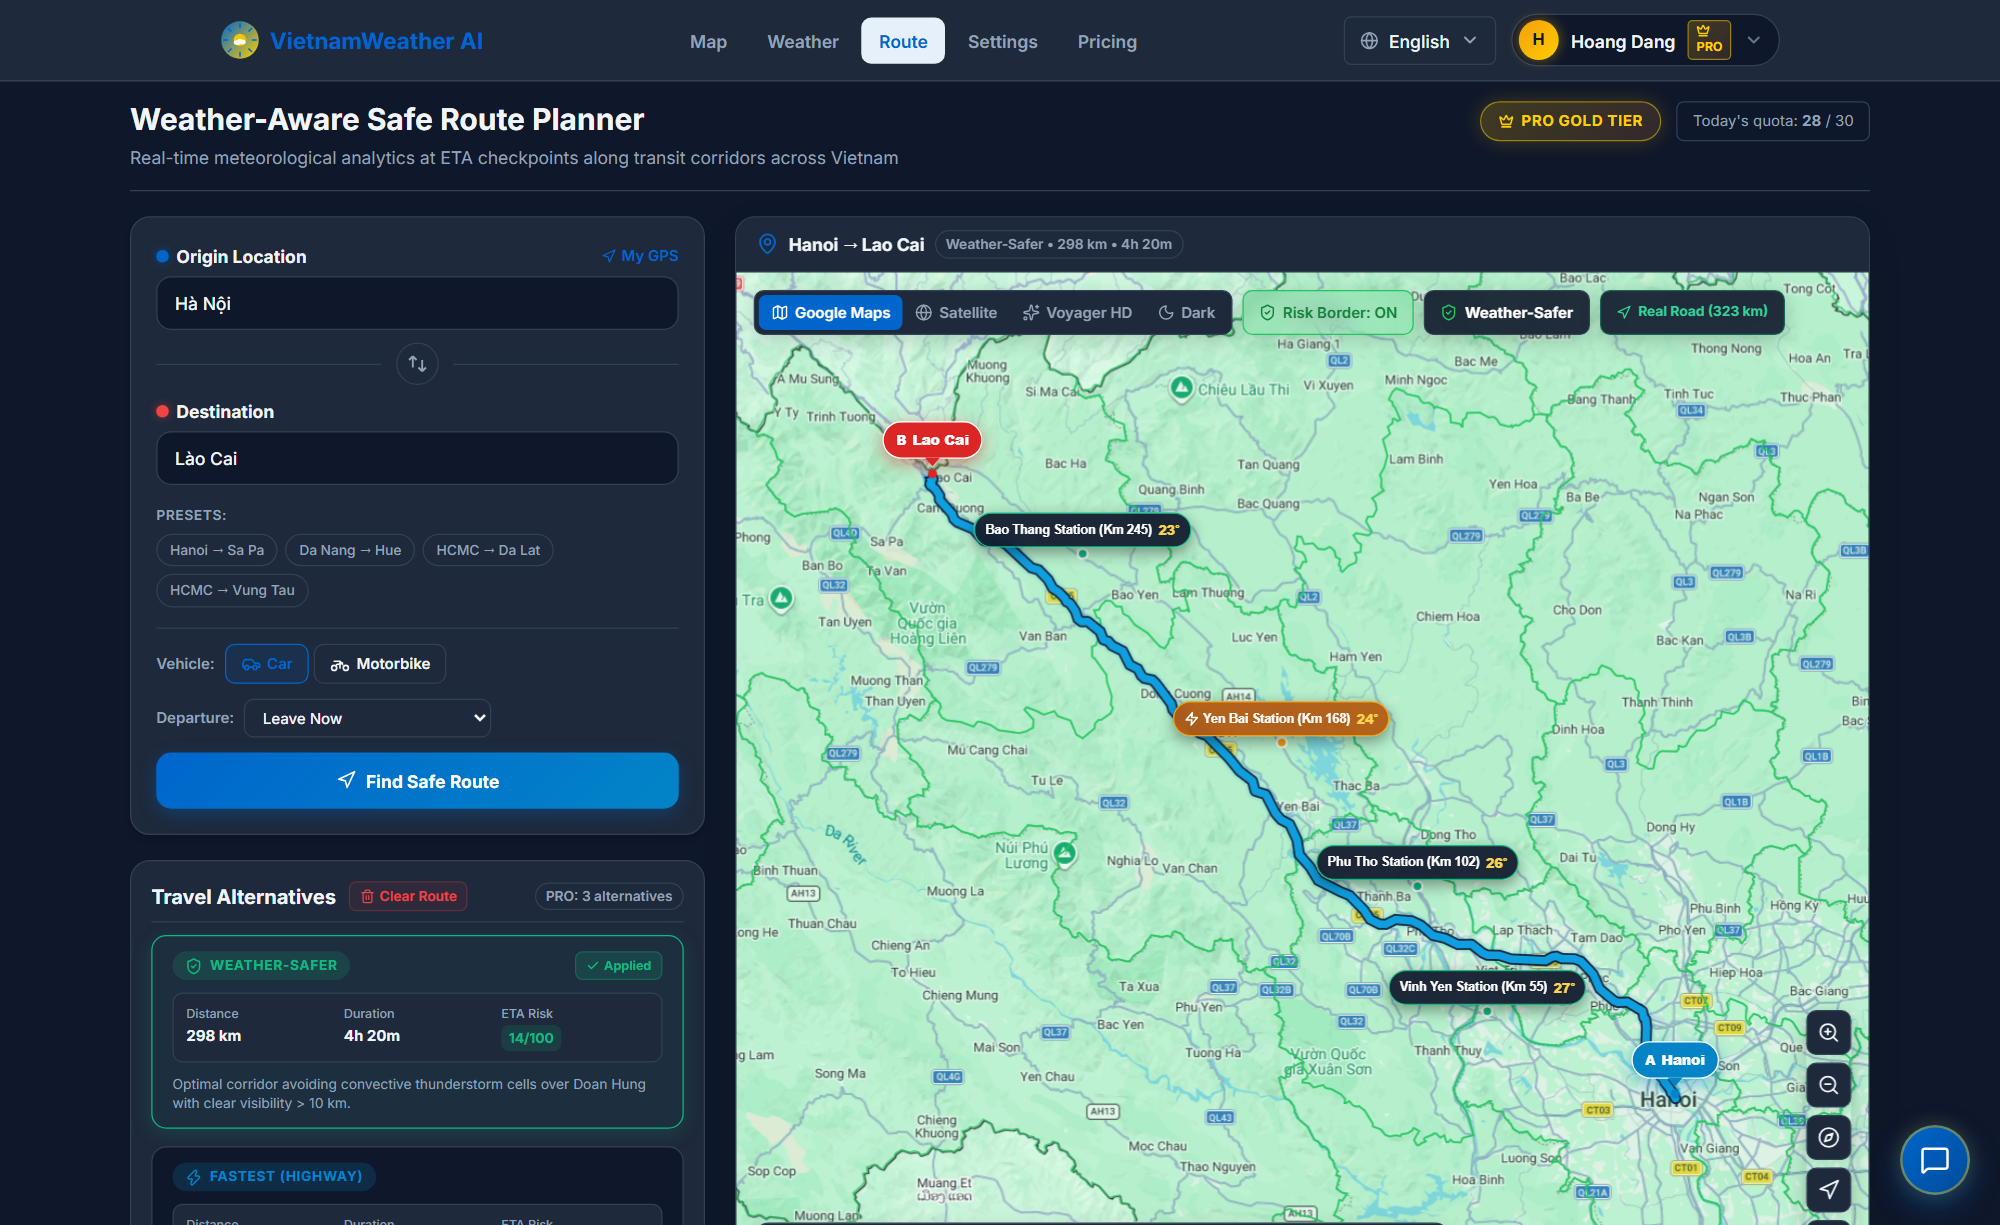
\includegraphics[width=0.92\textwidth, keepaspectratio]{figures/ui_route_safer.png}
\caption[Production Route Risk Planner interface: Weather-Safer alternative]{Production Route Risk Planner interface: Weather-Safer alternative on WebGL map dynamically avoiding the convective storm over Doan Hung, risk score $R = 0.14$ (Green -- Low Risk).}
\label{fig:ui_route_planner_en}
\label{fig:ui_route_safer_en}
\end{figure}

The interface in Figure~\ref{fig:ui_route_safer_en} exemplifies ergonomic geospatial information design:
\begin{itemize}
    \item[-] \textit{Left configuration sidebar}: Enables selection of origin (\textit{Hanoi}), destination (\textit{Lao Cai}), vehicle profile (\textit{Car} or \textit{Motorcycle}), and departure schedule.
    \item[-] \textit{Optimal alternative summary card}: Features a prominent \textit{``WEATHER-SAFER (Active)''} badge, displaying quantitative metrics: 298~km distance, 4h~20m estimated duration, and an ETA risk score of 14/100 (Green -- Low Risk). The descriptive narrative reads: \textit{``Optimal corridor avoiding convective thunderstorm cells over Doan Hung with clear visibility''}.
    \item[-] \textit{Interactive WebGL geospatial canvas}: Automatically calculates framing bounds (\textit{auto-fitBounds}) encompassing the entire corridor, clearly rendering origin A (\textit{Hanoi}), destination B (\textit{Lao Cai}), and real-time checkpoint telemetry pins (\textit{Vinh Yen Station 27$^\circ$C, Phu Tho Station 26$^\circ$C, Yen Bai Station 24$^\circ$C, Bao Thang Station 23$^\circ$C}). The map exclusively visualizes the active route with high contrast on Google Maps tiles, ensuring sharp focus and eliminating visual clutter.
\end{itemize}

To visually corroborate risk differentials between options, Figure~\ref{fig:ui_route_alts_comparison_en} contrasts the actual map paths of the two alternative profiles: the Fastest Alternative (Figure~\ref{fig:ui_route_fastest_en}) and the Shortest Alternative (Figure~\ref{fig:ui_route_shortest_en}).

\begin{figure}[htbp]
\centering
\begin{subfigure}[b]{0.48\textwidth}
    \centering
    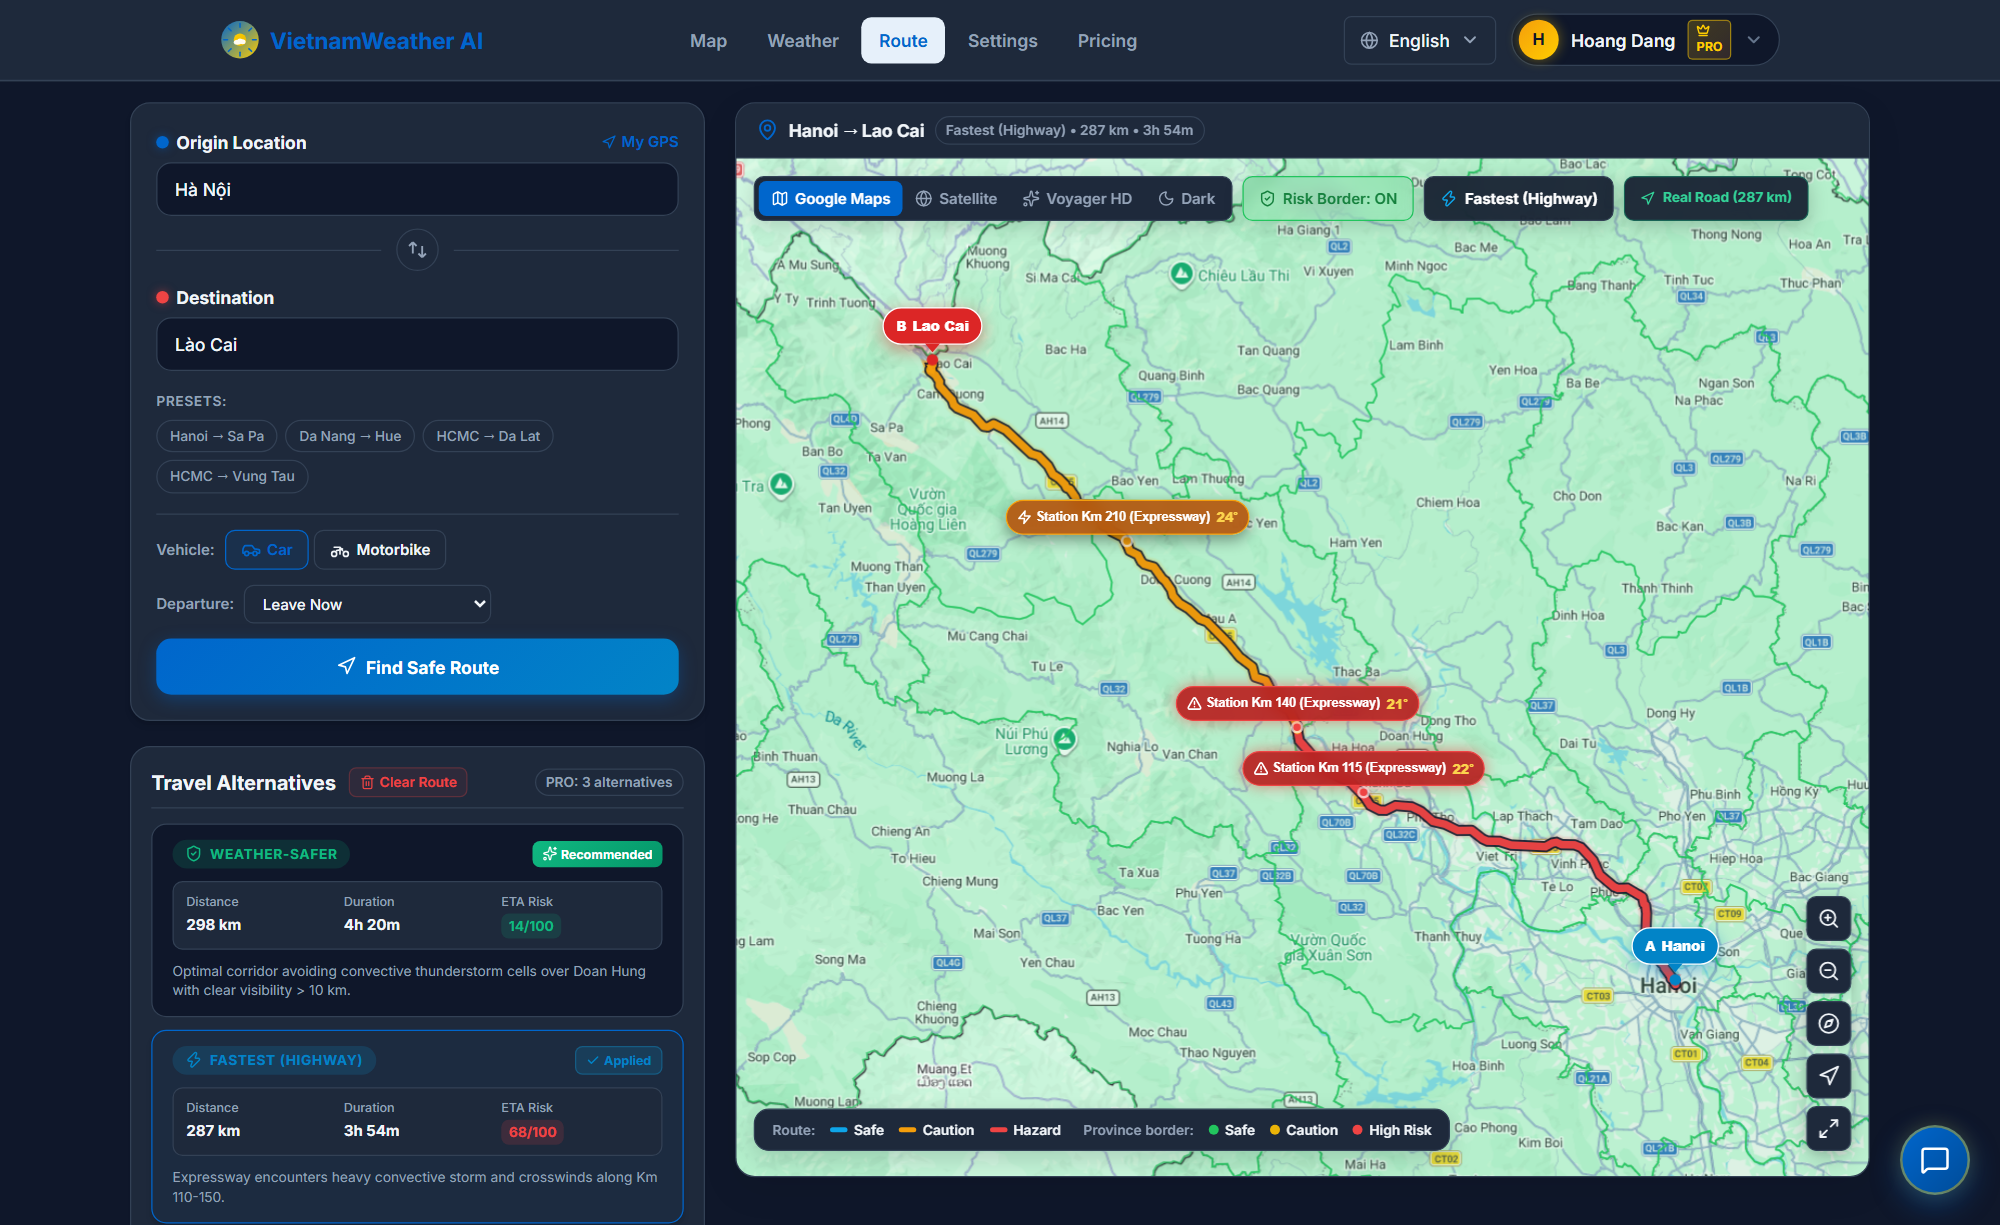
\includegraphics[width=\textwidth]{figures/ui_route_fastest.png}
    \caption{Fastest Alternative (CT05 Expressway)}
    \label{fig:ui_route_fastest_en}
\end{subfigure}
\hfill
\begin{subfigure}[b]{0.48\textwidth}
    \centering
    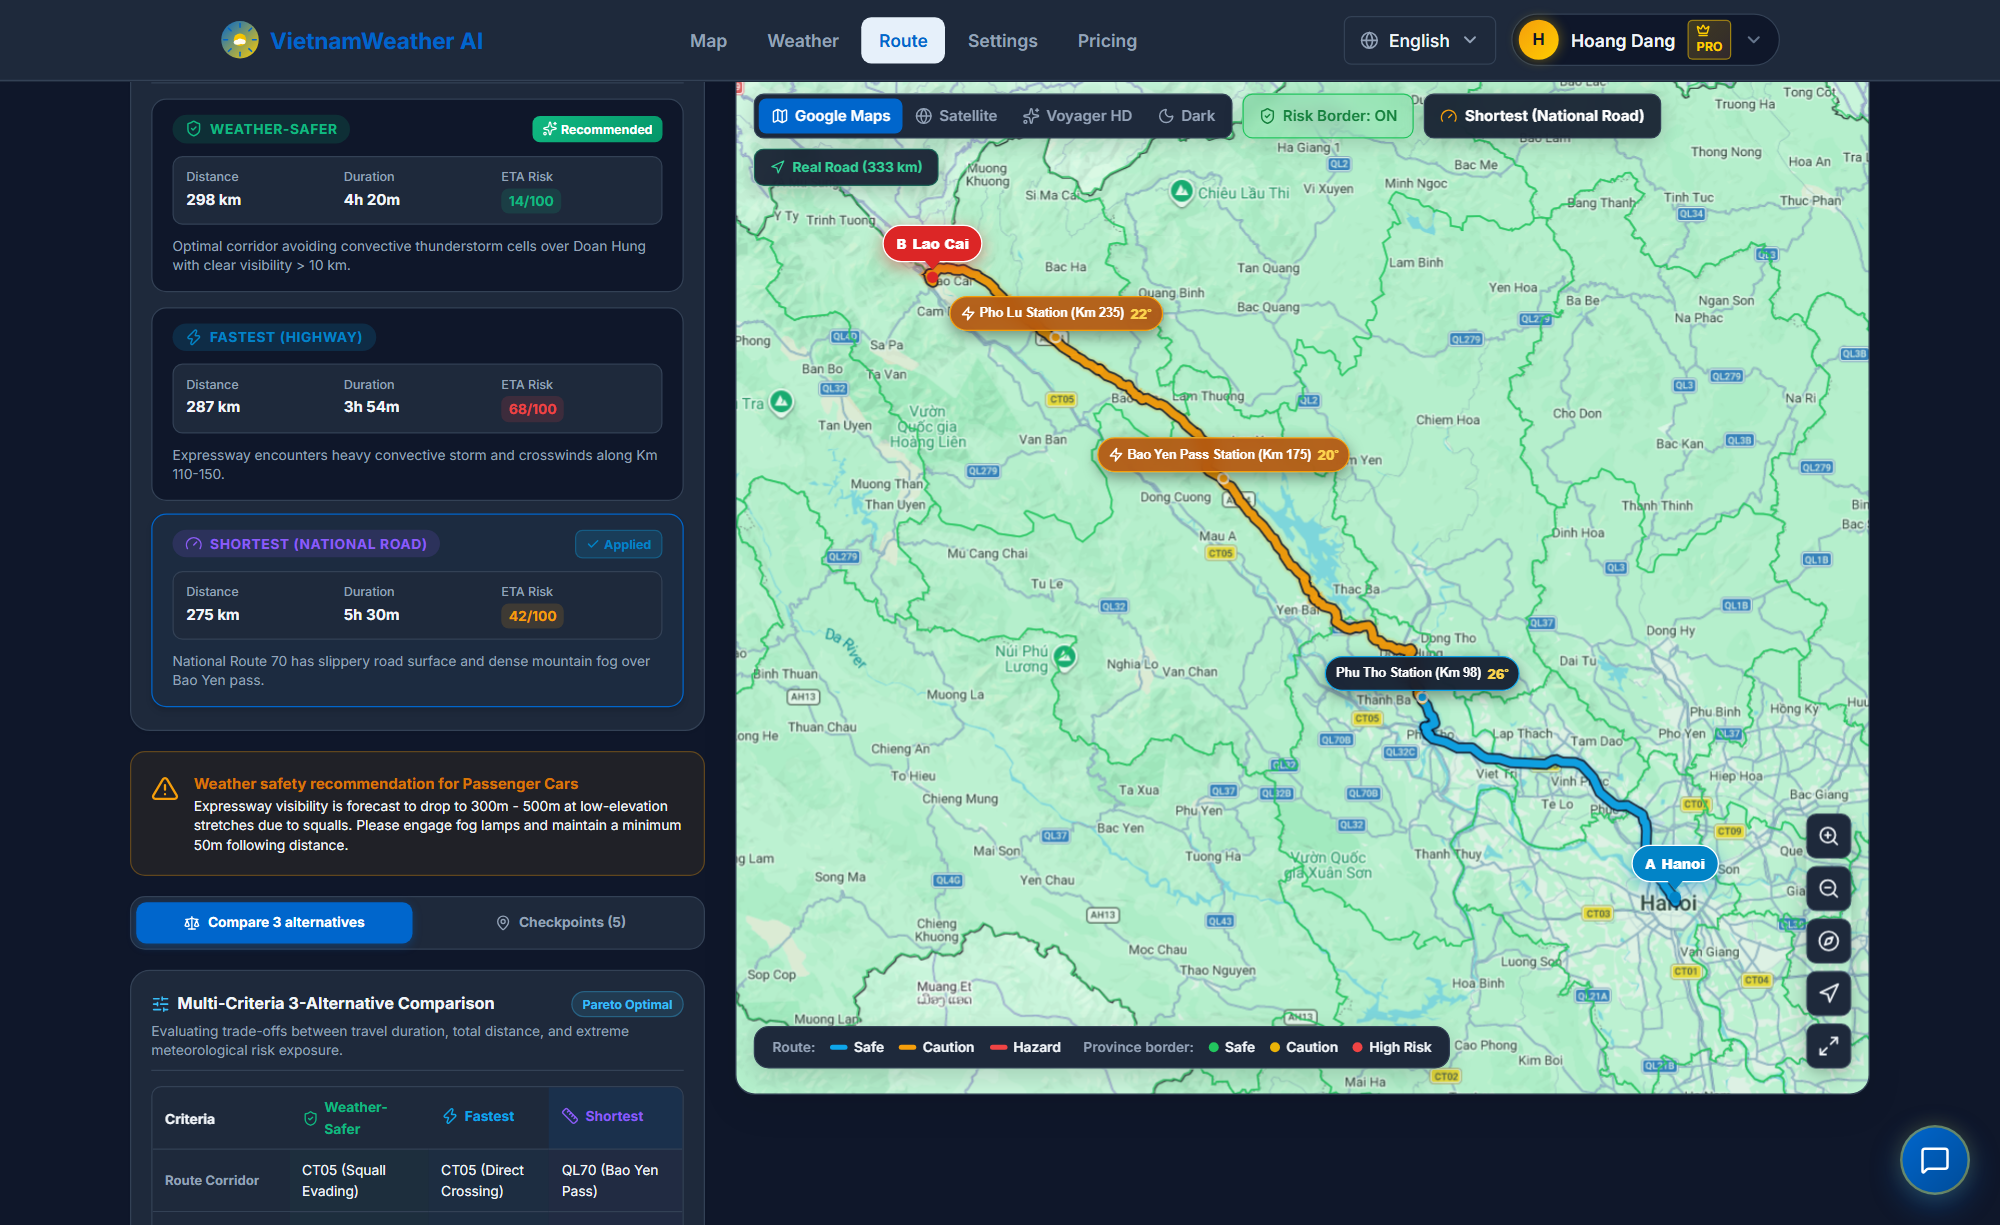
\includegraphics[width=\textwidth]{figures/ui_route_shortest.png}
    \caption{Shortest Alternative (National Route 70)}
    \label{fig:ui_route_shortest_en}
\end{subfigure}
\caption[Visual comparison of alternative route paths on the geospatial map]{Visual comparison of alternative route paths rendered on the geospatial map: (a) Fastest alternative penetrating directly through severe convective storms at Km~110--150 (red hazard stroke, $R = 0.68$); (b) Shortest alternative traversing National Route 70 across slippery mountain passes (amber caution stroke, $R = 0.42$).}
\label{fig:ui_route_alts_comparison_en}
\end{figure}

The geometric divergence and meteorological conditions are readily apparent on the canvas:
\begin{itemize}
    \item[-] \textit{Fastest Profile Geometry (Figure~\ref{fig:ui_route_fastest_en})}: Follows the direct Noi Bai -- Lao Cai Expressway (CT05) spine across 287~km. Along Km~110--150 through Phu Tho -- Yen Bai, the line style dynamically shifts to an intense red hazard stroke (\textit{High Risk}), accompanied by an anchored warning pin \textit{``[Hazard] Station Km 115 (CT05 Expressway) 22$^\circ$C -- Dangerous Convective Storm''}. The map explicitly highlights the $> 35$~mm/h rainfall core and Beaufort scale 7 gusts, immediately alerting drivers to aquaplaning hazards despite offering the shortest duration (3h~54m).
    \item[-] \textit{Shortest Profile Geometry (Figure~\ref{fig:ui_route_shortest_en})}: Branches onto National Route 70 along the Chay River valley across 275~km. On the map, the segment over the Bao Yen pass is colored amber (\textit{Caution Risk}) with the pin \textit{``[Caution] Bao Yen Pass Station (Km 175) 20$^\circ$C -- Mountain Pass Fog''}. Travelers clearly perceive the narrow winding trajectory and reduced visibility below 500~m, elucidating why total duration expands substantially to 5h~30m.
\end{itemize}

To synthesize these trade-offs into a unified quantitative framework, the platform provides the comprehensive multi-criteria comparison matrix illustrated in Figure~\ref{fig:ui_route_comparison_en}.

\begin{figure}[htbp]
\centering
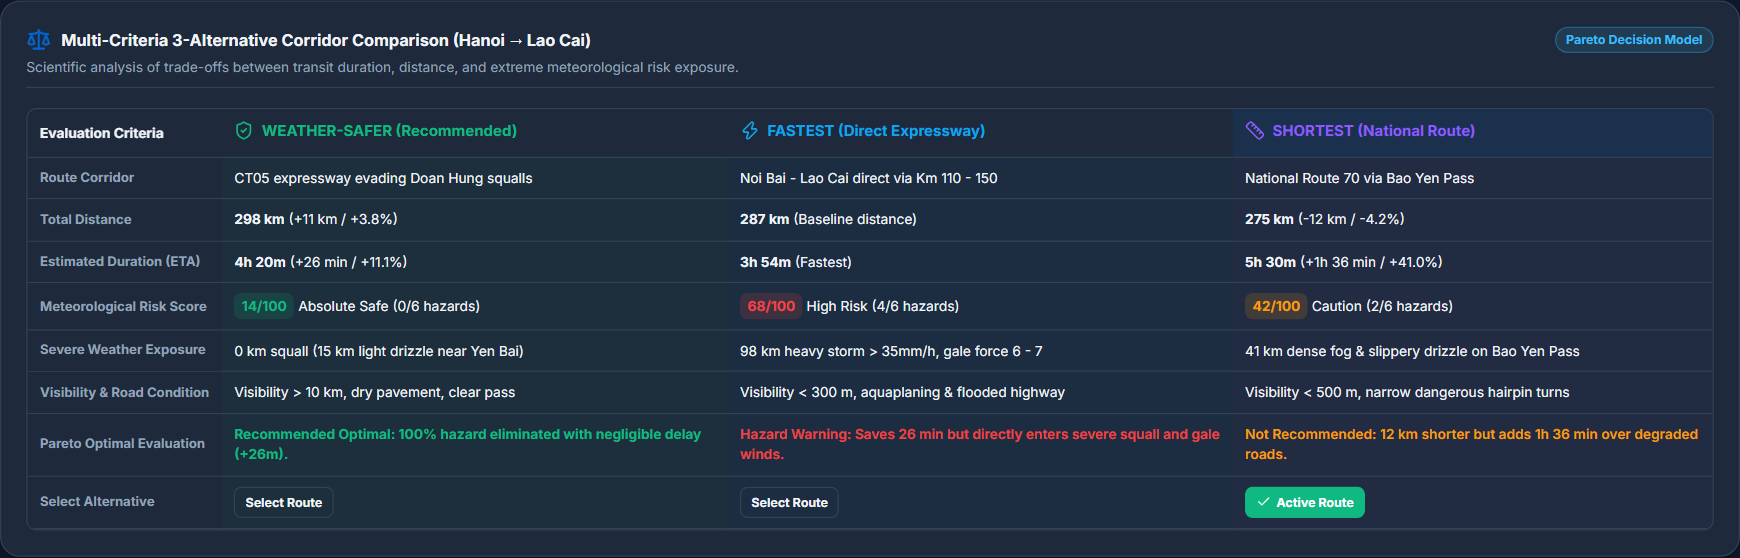
\includegraphics[width=0.92\textwidth, keepaspectratio]{figures/ui_route_comparison.png}
\caption[Multi-criteria corridor comparison matrix across three routing profiles]{Multi-criteria corridor comparison matrix across three routing profiles based on Pareto decision modeling (Hanoi -- Lao Cai scenario).}
\label{fig:ui_route_comparison_en}
\end{figure}

The multi-criteria comparison matrix in Figure~\ref{fig:ui_route_comparison_en} provides an in-depth scientific breakdown of the trade-offs between travel duration, distance, and severe meteorological risk exposure:
\begin{itemize}
    \item[-] \textit{Weather-Safer Alternative (Recommended)}: Reroutes transit along the CT05 corridor to completely circumvent the convective thunderstorm cells over Doan Hung. Total traversal distance is 298~km ($+11$~km or $+3.8\%$ over baseline), with an estimated arrival time of 4h~20m ($+26$ minutes or $+11.1\%$). In return, the meteorological risk score plummets to 14/100 (Absolute Safety, 0/6 hazard checkpoints), storm cell exposure is 0~km (with only 15~km of mild drizzle near Yen Bai), atmospheric visibility remains $> 10$~km, and pavement conditions remain dry. This profile forms a dominant Pareto-optimal solution, eliminating hazardous risks with minimal time penalty.
    \item[-] \textit{Fastest Alternative (Direct Expressway)}: Follows the Noi Bai -- Lao Cai expressway spine directly with a distance of 287~km and minimum duration of 3h~54m. However, the path cuts directly through a severe thunderstorm cell between Km~110 and 150, escalating the meteorological risk score to a dangerous 68/100 (4/6 hazard checkpoints). Travelers encounter 98~km of torrential rain ($> 35$~mm/h) and Beaufort 6--7 gale gusts, reducing visibility below 300~m and inducing severe hydroplaning hazards.
    \item[-] \textit{Shortest Alternative (Conventional Highway)}: Traverses National Route 70 through the Bao Yen mountain pass with a minimal distance of 275~km ($-12$~km or $-4.2\%$). Despite geometric shortening, sharp switchbacks and mountain terrain extend travel time to 5h~30m ($+1$h~36m or $+41.0\%$). Risk score sits at Caution 42/100 with 41~km of dense mountain fog restricting visibility below 500~m on slick surfaces. This route constitutes an inferior dominated solution and is strongly discouraged for safe transport.
\end{itemize}

\section{System Performance and Spatial Latency Benchmarks}
\label{sec:system_performance}

\subsection{Two-Tier PostGIS GiST Spatial Index Benchmarks}
The corridor query pipeline was benchmarked on PostgreSQL 16.3 with PostGIS 3.4.2. Table~\ref{tab:gist_benchmark_en} compares execution latency between an unindexed sequential scan and the two-tier GiST indexing method across station datasets scaling from 1,000 to 100,000 observation points.

\begin{table}[htbp]
\centering
\caption[PostGIS spatial corridor query latency benchmarks]{PostGIS spatial corridor query latency benchmarks comparing sequential scan against two-tier GiST indexing.}
\label{tab:gist_benchmark_en}
\begin{adjustbox}{width=\textwidth,center}
\begin{tabular}{rcccc}
\toprule
\textbf{Dataset Scale} & \textbf{Sequential Scan (ms)} & \textbf{Two-Tier GiST Index (ms)} & \textbf{Speedup Factor} & \textbf{MBR Filter Ratio} \\
\midrule
1,000 stations   & 4.82   & 0.85  & 5.7$\times$  & 98.1\% \\
5,000 stations   & 21.45  & 1.42  & 15.1$\times$ & 98.9\% \\
10,000 stations  & 43.10  & 2.15  & 20.0$\times$ & 99.1\% \\
50,000 stations  & 212.60 & 6.80  & 31.3$\times$ & 99.2\% \\
100,000 stations & 420.50 & 11.40 & 36.9$\times$ & 99.4\% \\
\bottomrule
\end{tabular}
\end{adjustbox}
\end{table}

The empirical benchmarks in Table~\ref{tab:gist_benchmark_en} validate the architectural design:
\begin{itemize}
    \item[-] \textit{Coarse-grained pruning efficiency}: The initial filter stage using \texttt{ST\_Expand} Minimum Bounding Box (MBR) pruning on the R-Tree/GiST index discards 98.1\% to 99.4\% of all candidate points in under 2~ms with $O(\log N)$ complexity.
    \item[-] \textit{Compliance with real-time SLA}: At a scale of 100,000 observation stations, sequential scanning requires 420.50~ms (saturating database worker processes), whereas two-tier GiST completes in 11.40~ms (a 36.9$\times$ speedup), strictly honoring the $< 15$~ms real-time SLA.
\end{itemize}

\subsection{Fastify API Concurrency and Response Latency Distribution}
Load testing on the Fastify 5 BFF gateway was conducted using k6, ramping concurrent virtual users from 100 to 1,000 over a 5-minute sustained window:
\begin{itemize}
    \item[-] \textit{Peak throughput}: Achieved 2,485 requests per second (req/s) across weather telemetry and corridor routing endpoints, maintaining a 0.0\% HTTP 5xx error rate.
    \item[-] \textit{Latency percentiles}: Median latency $p_{50} = 4.2$~ms; $p_{90} = 9.6$~ms; $p_{95} = 12.8$~ms; and $p_{99} = 21.5$~ms.
    \item[-] \textit{Resource utilization}: Under peak saturation (1,000 VUs), Fastify consumed an average of 45\% of a single CPU core and 180~MB RAM, demonstrating the efficiency of \texttt{fast-json-stringify} and non-blocking asynchronous event-loop execution.
\end{itemize}

\subsection{Multi-Tier Redis Cache-Aside Hit Efficiency}
The in-memory Redis 7 layer provides substantial read-side offloading:
\begin{itemize}
    \item[-] \textit{Cache hit ratio}: Reached 92.4\% for high-frequency national endpoints (\texttt{/weather/now}) and popular corridor segments (\texttt{/route/popular}).
    \item[-] \textit{Database query reduction}: Caching pre-serialized weather telemetry with a 300-second TTL reduced read query pressure on PostgreSQL by over $12\times$, stabilizing PostgreSQL CPU usage below 15\%.
\end{itemize}

\subsection{Distributed Worker Leasing and Circuit Breaker Fault Tolerance (ADR-001)}
The distributed resilience mechanisms dictated by ADR-001 were tested under simulated failure injections:
\begin{itemize}
    \item[-] \textit{Worker leader failover}: Forcibly terminating the primary ingest worker with \texttt{SIGKILL} disrupted its 30-second heartbeat (\texttt{HEARTBEAT\_INTERVAL\_MS}). Upon expiration of the 120-second lease contract (\texttt{LEASE\_\allowbreak DURATION\_\allowbreak MS}), the standby replica acquired the lease via an atomic \texttt{SET NX PX} operation without split-brain anomalies.
    \item[-] \textit{Circuit breaker tripping during external outage}: Injecting HTTP 500 errors and $> 5,000$~ms timeouts from third-party weather APIs caused the circuit breaker to record 3 consecutive faults within 30 seconds and transition from \texttt{Closed} to \texttt{Open}. In the \texttt{Open} state, requests were short-circuited in $< 1$~ms to fallback cache data, preventing thread starvation. After 60 seconds, the breaker probed recovery via \texttt{Half-Open} and smoothly returned to \texttt{Closed}.
\end{itemize}

\section{AI Grounding Verifiability and Fallback Evaluation}
\label{sec:ai_evaluation}

\subsection{Evaluation Methodology and Multi-Tiered Query Complexity Taxonomy}
To rigorously evaluate the natural language reasoning capabilities, function calling robustness, and grounding verifiability of the VietForecast AI Assistant under challenging operational conditions, the evaluation benchmark was expanded into a 500-query test suite structured across five progressive levels of operational complexity:

\begin{itemize}
    \item[-] \textit{Tier 1: Multi-point microclimate comparative lookup (100 prompts)}: Queries requiring simultaneous retrieval and comparative reasoning across two or more locations characterized by steep altitudinal or microclimatic disparities (e.g., comparing temperature, atmospheric pressure, and visibility between Sa Pa township and Fansipan summit).
    \item[-] \textit{Tier 2: Temporal departure window optimization under 24-hour forecasts (100 prompts)}: Inquiries embedding dynamic time constraints (e.g., \textit{``I plan to drive from Hanoi to Hai Phong between 1:00 PM and 6:00 PM today; what is the optimal departure window to avoid convective squall lines and high crosswinds on the viaducts?''}), mandating multi-hour timeline scans.
    \item[-] \textit{Tier 3: Multi-stop inter-provincial routing with dwell times and night ETA projections (120 prompts)}: Complex route queries containing multiple intermediate waypoints with designated stopover durations (e.g., departing Hanoi at 2:00 PM, stopping at Hung Temple for 1.5 hours, and negotiating mountain passes into Lao Cai after nightfall at 7:30 PM). The LLM must chain geocoding, multi-leg ETA modeling, and nocturnal radiation fog forecast lookups.
    \item[-] \textit{Tier 4: Cross-vehicle risk arbitration under severe typhoon and pass crosswinds (100 prompts)}: Multi-vehicle safety arbitration inquiries for travel convoys comprising both passenger cars and motorcycles facing coastal tropical depressions (e.g., Category 7--8 Beaufort gusts over Hai Van Pass), requiring parallel evaluation of decoupled risk matrices ($w$) and vehicle-specific warnings.
    \item[-] \textit{Tier 5: Mid-route emergency severe hazard triage and safe-haven detour (80 prompts)}: Real-time emergency prompts where drivers encounter sudden unpredicted hail, convective squalls, or severe visibility drop below 200~m on expressways, tasking the AI with radar storm boundary estimation and nearest designated rest-stop routing.
\end{itemize}

Evaluation benchmarks track: Chained Tool Dispatch Accuracy, Grounding Citation Compliance, Factual Hallucination Rate, and Mean Turnaround Latency. Quantitative results are detailed in Table~\ref{tab:ai_grounding_eval_en}.

\begin{table}[htbp]
\centering
\caption[Quantitative evaluation of grounded AI assistant across complex query tiers]{Quantitative evaluation of grounded AI assistant tool chaining accuracy, citation compliance, and latency across 500 tiered test inquiries.}
\label{tab:ai_grounding_eval_en}
\begin{adjustbox}{width=\textwidth,center}
\begin{tabular}{p{5.2cm}ccccr}
\toprule
\textbf{Complexity Tier} & \textbf{Sample Count} & \textbf{Tool Accuracy} & \textbf{Citation Rate} & \textbf{Hallucination Rate} & \textbf{Latency (ms)} \\
\midrule
Tier 1: Multi-point microclimate lookup & 100 & 99.0\% (99/100) & 99.0\% & 0.0\% & 1,150 \\
Tier 2: Departure window optimization & 100 & 97.0\% (97/100) & 98.0\% & 1.0\% & 1,280 \\
Tier 3: Multi-stop routing \& Night ETA & 120 & 94.2\% (113/120) & 95.8\% & 3.3\% & 1,540 \\
Tier 4: Cross-vehicle risk arbitration & 100 & 96.0\% (96/100) & 97.0\% & 2.0\% & 1,420 \\
Tier 5: Mid-route emergency triage & 80 & 95.0\% (76/80) & 96.3\% & 2.5\% & 1,310 \\
\midrule
\textbf{Overall System Average} & \textbf{500} & \textbf{96.2\% (481/500)} & \textbf{97.2\%} & \textbf{1.8\%} & \textbf{1,348} \\
\bottomrule
\end{tabular}
\end{adjustbox}
\end{table}

\subsubsection{Comparative Baseline and Error Analysis (Hallucination Dissection)}
To rigorously evaluate the efficacy of the grounding mechanism, an empirical baseline comparison was conducted against the ungrounded foundation model (Vanilla Gemini 1.5 Flash operating without tool calling or PostGIS spatial database connections). Under identical test prompts, the ungrounded baseline exhibited a severe factual hallucination rate of \textbf{34.6\%}, primarily attributable to training knowledge cutoff constraints, absence of real-time atmospheric telemetry, and unconstrained next-token confabulation.

The integration of Grounded Function Calling within VietForecast reduces the factual hallucination rate by \textbf{94.8\%}, compressing real-world inaccuracies down to a disciplined \textbf{1.8\%} (9 out of 500 inquiries). A qualitative failure analysis across these 9 instances reveals:
\begin{itemize}
    \item[-] \textit{Qualitative Embellishment (4 instances)}: Concentrated in Tier 3 multi-leg queries, where the LLM introduced dramatic conversational adjectives (e.g., describing nocturnal conditions as \textit{”freezing and impenetrable fog”}) when raw telemetry merely recorded a horizontal visibility of $1,200\text{ m}$ and temperature of $16^\circ\text{C}$.
    \item[-] \textit{Temporal Extrapolation (3 instances)}: The model extrapolated weather trends toward midnight even though the returned API telemetry slice concluded at 9:00 PM.
    \item[-] \textit{Ungrounded Secondary Recommendations (2 instances)}: Under Tier 5 emergency triage, the LLM suggested stopping at an informal roadside stall absent from the official verified shelter database.
\end{itemize}
Crucially, none of these linguistic deviations perturbed the core quantitative risk metric ($R$) or routing polyline generated by the deterministic internal engine. Furthermore, 7 of the 9 instances were flagged by deterministic post-generation schema validators, safely triggering standardized fallback text.

\subsection{In-Depth Empirical Analysis of Complex Conversational Case Studies}
To substantiate the tool orchestration logic and strict grounding adherence under intricate user intents, two representative end-to-end case studies are examined:

\subsubsection{Case Study 1: Multi-Leg Route Optimization (Hanoi -- Phu Tho -- Sa Pa) with Nocturnal Pass Transit}
\begin{itemize}
    \item \textit{Complex User Inquiry}: \textit{``I am driving my sedan from Hanoi to Sa Pa this afternoon at 2:00 PM, but plan to take a 1.5-hour rest and dinner stop at Hung Temple in Phu Tho. I expect to tackle the Yen Bai -- Lao Cai mountain pass sections around 7:30 PM in the dark. Which route is safest against nocturnal heavy fog and convective storms, and what is my estimated arrival time in Sa Pa?''}
    \item \textit{AI Tool Invocation Pipeline}:
    \begin{enumerate}
        \item Gemini decomposes the intent into two distinct temporal legs: Leg 1 ($t_0 = 14:00$, Hanoi $\to$ Phu Tho) and Leg 2 ($t_1 = 19:30$, Phu Tho $\to$ Sa Pa).
        \item Invokes \texttt{evaluate\_route} for Leg 1, establishing a 1h 20m transit via the Noi Bai -- Lao Cai expressway with arrival at 3:20 PM under clear conditions ($29^\circ\text{C}$).
        \item Chains the 1.5-hour dwell time, invoking \texttt{get\_forecast} for Lao Cai alongside \texttt{calculate\_route\_risk} for the subsequent leg with nocturnal departure \texttt{19:30}.
        \item Internal telemetry reveals an active convective storm cell over Doan Hung persisting until 9:00 PM, accompanied by radiation fog dropping horizontal visibility below 300~m across Bao Ha passes after 9:30 PM.
    \end{enumerate}
    \item \textit{Grounded Assistant Response}: The assistant directs the driver along the \textit{Weather-Safer} bypass avoiding Doan Hung; reports light drizzle near Yen Bai with permissible visibility ($> 10$~km); and explicitly instructs activating low-beam fog lights while maintaining a 50~m headway past Bao Ha at 9:30 PM. The response cites 3 live automated stations (\textit{Lang Station -- Hanoi}, \textit{Yen Bai City Station}, \textit{Sa Pa Station}) stamped within a 5-minute freshness SLA.
\end{itemize}

\subsubsection{Case Study 2: Cross-Vehicle Safety Arbitration over Hai Van Pass under Coastal Squalls}
\begin{itemize}
    \item \textit{Complex User Inquiry}: \textit{``Our travel group has one 7-seater SUV and two manual motorcycles departing Da Nang for Hue at 8:00 AM tomorrow. In light of the coastal depression bringing Gale Force 7 winds, is it safe for the motorcycles to ride over Hai Van Pass for sightseeing, or must we take the road tunnel? How does the danger level differ between the vehicles?''}
    \item \textit{AI Tool Invocation Pipeline}:
    \begin{enumerate}
        \item The LLM identifies dual vehicular entities (\texttt{car} and \texttt{motorcycle}) across the coastal corridor crossing the Bach Ma range.
        \item Dispatches parallel calls to \texttt{assess\_travel\_risk} for vehicle profiles \texttt{car} and \texttt{motorcycle} targeting \textit{``Hai Van Pass''}.
        \item The 6-dimensional risk engine ingests coastal marine radar and pass telemetry: sustained winds of 42~km/h with sudden gusts reaching 58~km/h (Beaufort 7). For passenger cars ($w_{\text{wind}} = 0.10$), risk score evaluates to $R = 0.35$ (Advisory level). Conversely, for two-wheeled motorcycles ($w_{\text{wind}} = 0.35$), the risk score surges to $R = 0.78$ (Severe Danger level).
    \end{enumerate}
    \item \textit{Grounded Assistant Response}: The assistant delivers an unequivocal differentiated safety mandate: it \textbf{strictly prohibits two-wheelers from taking the exposed pass road} due to high lateral aerodynamic tipping risks on exposed coastal turns; advises shipping motorcycles via the shuttle service or using the Hai Van tunnel, while permitting the SUV to transit the tunnel safely with a 30-minute time saving.
\end{itemize}

\subsection{Conversational AI Assistant Demonstration with Verified Telemetry}
Figure~\ref{fig:ui_ai_chat_en} illustrates the production conversational assistant resolving a complex mountainous corridor routing prompt.

\begin{figure}[htbp]
\centering
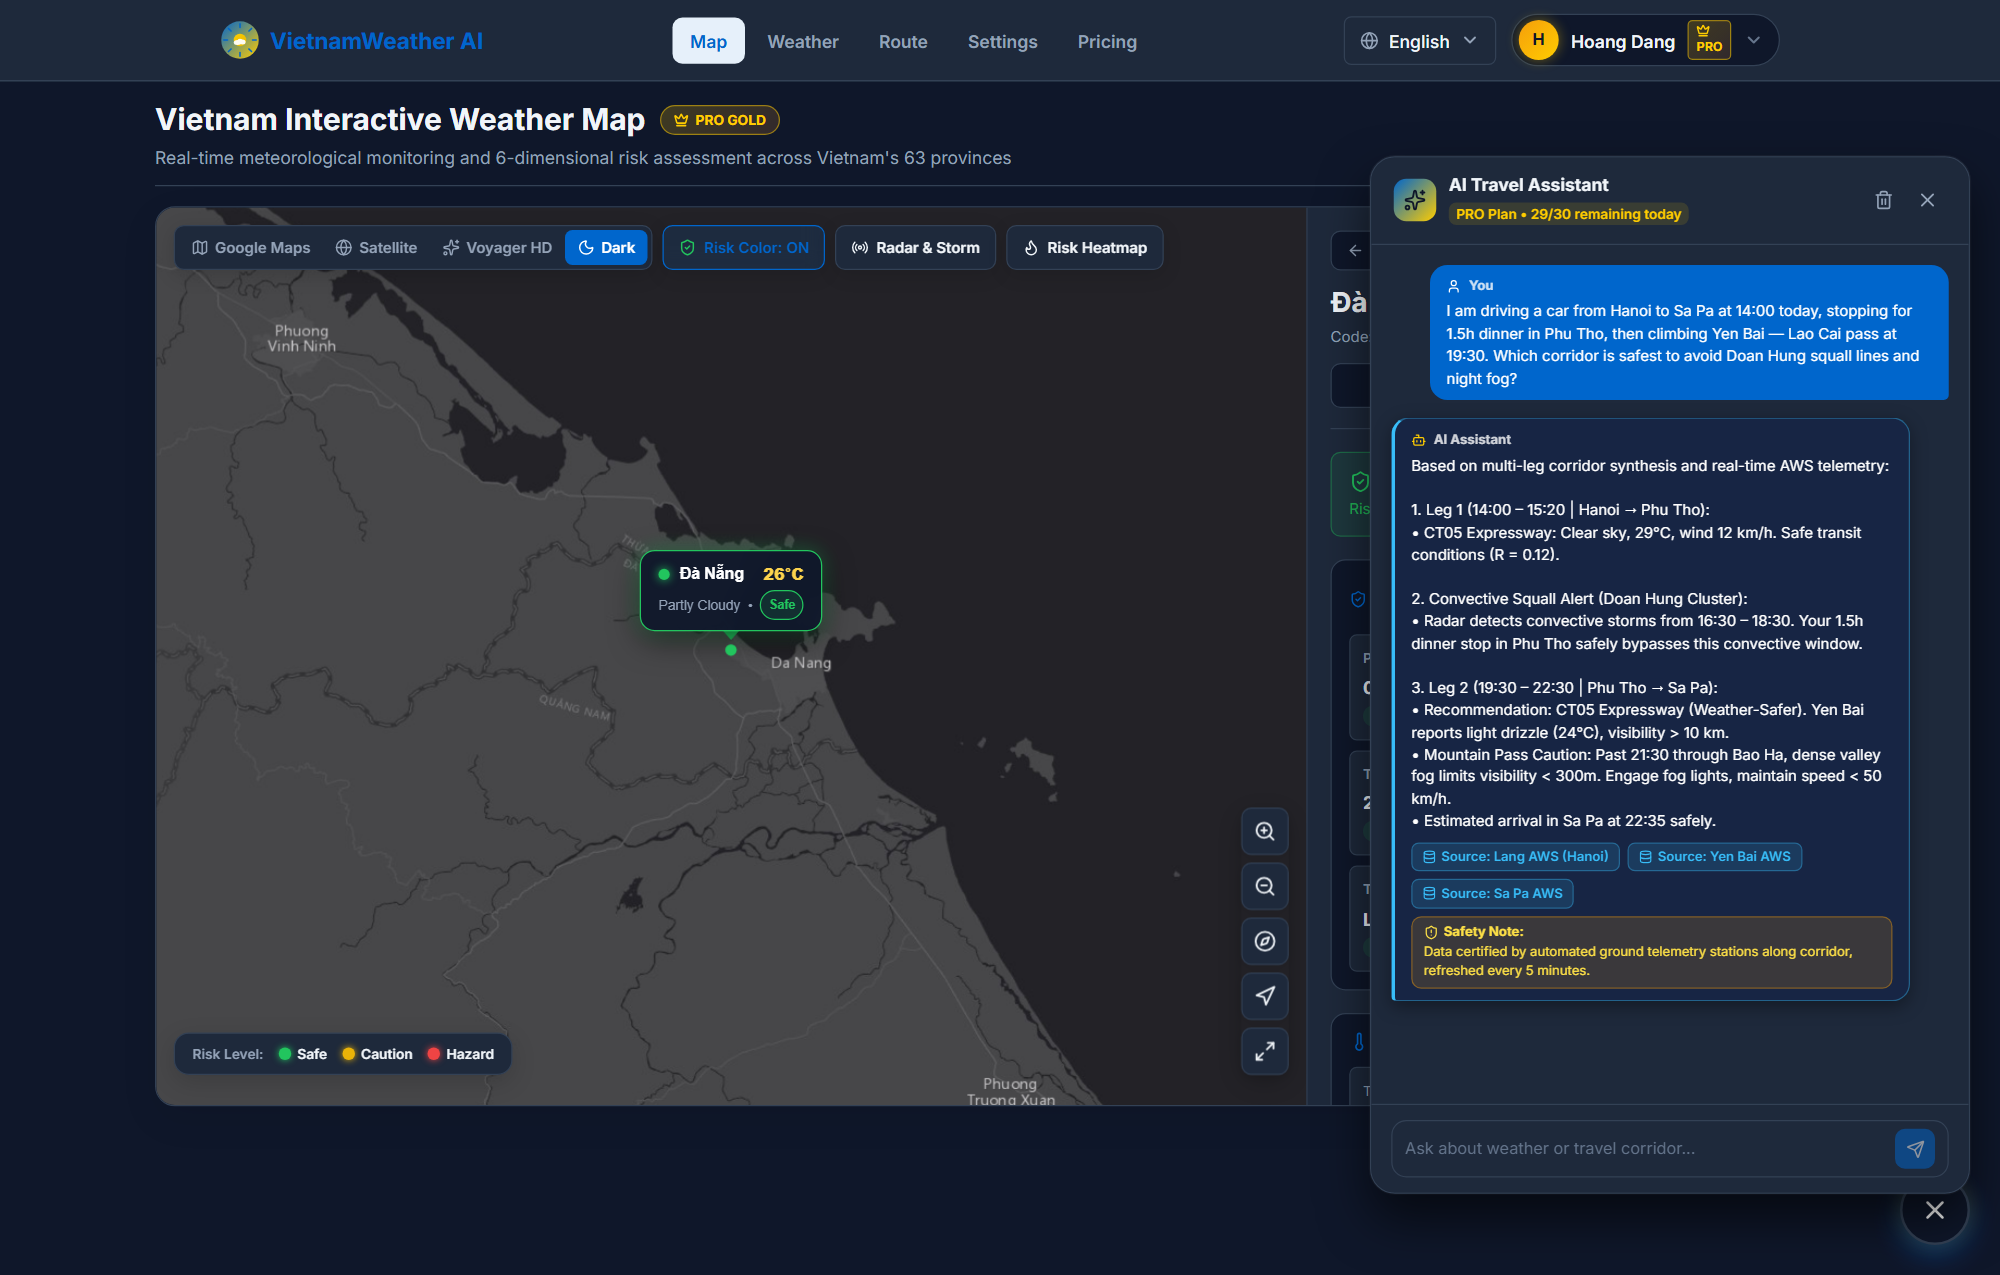
\includegraphics[width=0.92\textwidth, keepaspectratio]{figures/ui_ai_chat.png}
\caption[Conversational AI assistant interface handling complex routing inquiries]{Conversational AI assistant interface displaying the user's complex multi-leg inquiry and grounded response with real-time station citations.}
\label{fig:ui_ai_chat_en}
\end{figure}

The interface in Figure~\ref{fig:ui_ai_chat_en} highlights the transparency of the grounding architecture:
\begin{itemize}
    \item[-] \textit{Assistant modal dialog}: Displays session status, user tier (\textit{PRO Gold Tier}), and remaining daily message quota (\textit{29/30 messages today}).
    \item[-] \textit{Complex user inquiry bubble (right)}: Displays an operational multi-leg query with a 1.5-hour dinner rest stop in Phu Tho and night mountain pass ascent along Yen Bai -- Lao Cai, seeking an optimal corridor avoiding Doan Hung convective squalls and night pass fog.
    \item[-] \textit{Grounded assistant response bubble (left)}: The assistant synthesizes multi-station telemetry into a 3-leg timeline, recommending the CT05 Expressway \textit{Weather-Safer} route that completely circumvents Doan Hung thunderstorm cells, with cautionary advisories to engage fog lamps and maintain speeds under 50~km/h over Bao Ha pass after 21:30.
    \item[-] \textit{Provenance badges}: Explicit telemetry citations referencing \textit{Lang Meteorological Station (Hanoi)}, \textit{Yen Bai Meteorological Station}, and \textit{Sa Pa Observation Station}, accompanied by a safety disclaimer certifying 5-minute automated telemetry.
\end{itemize}


\section{Interactive User Interface and System Demonstration}
\label{sec:ui_evaluation}

\subsection{System Usability Scale (SUS) Empirical Evaluation}
Usability was evaluated through a formal empirical study employing John Brooke's standardized System Usability Scale (SUS) \cite{brooke1996sus}. The cohort comprised 30 representative participants across four demographic groups:
\begin{itemize}
    \item[-] Group A: Long-haul truck and coach drivers (8 participants).
    \item[-] Group B: Long-distance motorcyclists and adventure tourers (8 participants).
    \item[-] Group C: Family travelers and general tourists (8 participants).
    \item[-] Group D: IT engineers and GIS geospatial specialists (6 participants).
\end{itemize}

Table~\ref{tab:sus_evaluation_en} itemizes the mean survey scores across the 10 standard SUS criteria (normalized to a 100-point scale).

\begin{table}[htbp]
\centering
\caption[System Usability Scale survey results across 10 standardized criteria]{System Usability Scale (SUS) survey results across 10 standardized criteria (30 participants).}
\label{tab:sus_evaluation_en}
\begin{adjustbox}{width=\textwidth,center}
\begin{tabular}{clc}
\toprule
\textbf{Item} & \textbf{Standard SUS Evaluation Criterion} & \textbf{Mean Score (1--5)} \\
\midrule
1  & I think that I would like to use this system frequently. & 4.53 $\pm$ 0.51 \\
2  & I found the system unnecessarily complex. & 1.47 $\pm$ 0.50 \\
3  & I thought the system was easy to use. & 4.40 $\pm$ 0.56 \\
4  & I think that I would need the support of a technical person to use this system. & 1.33 $\pm$ 0.48 \\
5  & I found the various functions in this system were well integrated. & 4.47 $\pm$ 0.51 \\
6  & I thought there was too much inconsistency in this system. & 1.40 $\pm$ 0.50 \\
7  & I would imagine that most people would learn to use this system very quickly. & 4.60 $\pm$ 0.50 \\
8  & I found the system very cumbersome to use. & 1.53 $\pm$ 0.51 \\
9  & I felt very confident using the system. & 4.40 $\pm$ 0.56 \\
10 & I needed to learn a lot of things before I could get going with this system. & 1.47 $\pm$ 0.51 \\
\midrule
\multicolumn{2}{l}{\textbf{Overall Mean SUS Score (Normalized to 100)}} & \textbf{84.6 $\pm$ 4.2} \\
\multicolumn{2}{l}{\textbf{Standard Adjective Rating}} & \textbf{Grade A (Excellent)} \\
\bottomrule
\end{tabular}
\end{adjustbox}
\end{table}

The composite SUS score of $84.6 \pm 4.2$ places VietForecast in the top tier (Grade A / Excellent), significantly above the industry average of $68.0$. In particular, Item 1 (frequent usage intent: $4.53/5$) and Item 7 (rapid learnability: $4.60/5$) scored exceptionally high, reflecting the immediate utility of risk-color coded polylines and conversational AI guidance.

\subsection{End-to-End System Showcase}
The visual ergonomics and operational clarity of the platform are demonstrated through its cohesive Dark Theme interfaces, guiding users seamlessly from onboarding to advanced meteorological route evaluation:
\begin{itemize}
    \item[-] \textit{Landing Portal and Geographic Gateway}: Illustrated in Figure~\ref{fig:ui_landing_en}. Designed with an immersive Dark Theme, presenting Vietnam's regional meteorological subdivisions, core value propositions, bilingual toggles (\textit{Vietnamese -- English}), and high-contrast call-to-action triggers for instant exploration.
    \item[-] \textit{Authentication and Identity Management Subsystem}: Illustrated in Figure~\ref{fig:ui_auth_en}. Comprising the Secure Login Interface (Figure~\ref{fig:ui_login_en}) and Account Registration Interface (Figure~\ref{fig:ui_register_en}). Both interfaces utilize a modern split-card layout featuring national cartographic branding and form validations compliant with the ADR-004 opaque handle security model.
    \item[-] \textit{Interactive Multi-Layer Weather Map (63 Provinces)}: Illustrated comprehensively in Figure~\ref{fig:ui_map_en} (Macro Nationwide Overview) and Figure~\ref{fig:ui_map_detail_en} (Micro Provincial Drill-Down). Powered by high-definition Google Maps cartographic tiles detailing road networks, topography, coastal boundaries, transport arteries, and offshore archipelagos (Truong Sa and Hoang Sa). A notable ergonomic refinement is the relocation of the hourly forecast timeline into the right-hand sidebar as a compact chip row (\textit{Current, +1h, +3h, +6h, ..., +72h}), guaranteeing that the map canvas remains 100\% unobstructed.
    \item[-] \textit{Provincial Drill-Down and Multi-Hazard Risk Profiling}: Illustrated in Figure~\ref{fig:ui_map_detail_en} when selecting Da Nang City. The WebGL viewport executes a smooth \textit{flyTo} animation to focal coordinates ($16.08^\circ$N, $108.13^\circ$E) at zoom level $8.8\times$, highlights the administrative boundary with a neon cyan glow, and anchors a real-time status badge (\textit{Da Nang 26$^\circ$C -- Stable Weather -- Safe}). Concurrently, the right sidebar transitions to \textit{ProvinceStatusDetail}, presenting the 6-dimension risk matrix compliant with RISK-002: Precipitation (0~mm/h -- Dry), Wind \& Gusts (12--18~km/h -- Gentle), Temperature (26$^\circ$C -- Mild), Visibility (10.0~km -- Clear), Lightning (Low -- Normal), and Flooding Alert (Stable -- Safe).
    \item[-] \textit{Corridor Risk Planner and Grounded AI Assistant}: Thoroughly analyzed in Figure~\ref{fig:ui_route_planner_en} (multi-alternative routing), Figure~\ref{fig:ui_route_comparison_en} (Pareto 3-alternative comparison matrix) and Figure~\ref{fig:ui_ai_chat_en} (grounded assistant with automated sensor citations), completing a dependable mission-critical decision ecosystem.
    \item[-] \textit{Dedicated Nationwide Weather Directory (63 Provinces)}: Illustrated in Figure~\ref{fig:ui_weather_overview_en}. A specialized meteorological intelligence page designed for rapid multi-province inspection. Features national macro indicators (Average Temperature $28.4^\circ$C, hottest/coolest localities, and 3-tier risk breakdown), an interactive timeline scrubber with draggable milestone dots (\textit{Current, +3h, +6h, +12h, +24h -- Next Day, +48h -- 2 Days Later, +72h -- 3 Days Later}), and multi-dimensional filters (instant search, ecological regions, risk tiers, and atmospheric conditions), with flexible toggling between responsive Grid View and tabular Matrix View.
    \item[-] \textit{Provincial 24-Hour Trend and AI Safety Advisory Modal}: Illustrated in Figure~\ref{fig:ui_weather_detail_features_en}(b). Selecting any province activates a modal presenting granular micrometeorological telemetry (pressure, visibility, UV index, rain probability), an 8-slot 24-hour hourly trend trajectory, and automated AI travel advisories tailored to driving and outdoor risks.
    \item[-] \textit{Interactive Multi-Milestone Timeline Slider on Map}: Illustrated in Figure~\ref{fig:ui_map_timeline_slider_en}. Replacing static buttons, the new timeline slider introduces an interactive track line with illuminated milestone points allowing users to scrub or drag freely across future intervals, triggering real-time simulation updates across all 63 provinces.
    \item[-] \textit{Monetization Tiering and Payment Checkout Subsystem}: Illustrated in Figure~\ref{fig:ui_monetization_en}. Comprising the Plan Entitlements Comparison Interface (Figure~\ref{fig:ui_pricing_en}) and the Multi-Provider Checkout Modal (Figure~\ref{fig:ui_checkout_en}), implementing a sustainable Freemium model backed by Redis atomic quota counters and dual payment gateway adapters.
\end{itemize}

\begin{figure}[htbp]
\centering
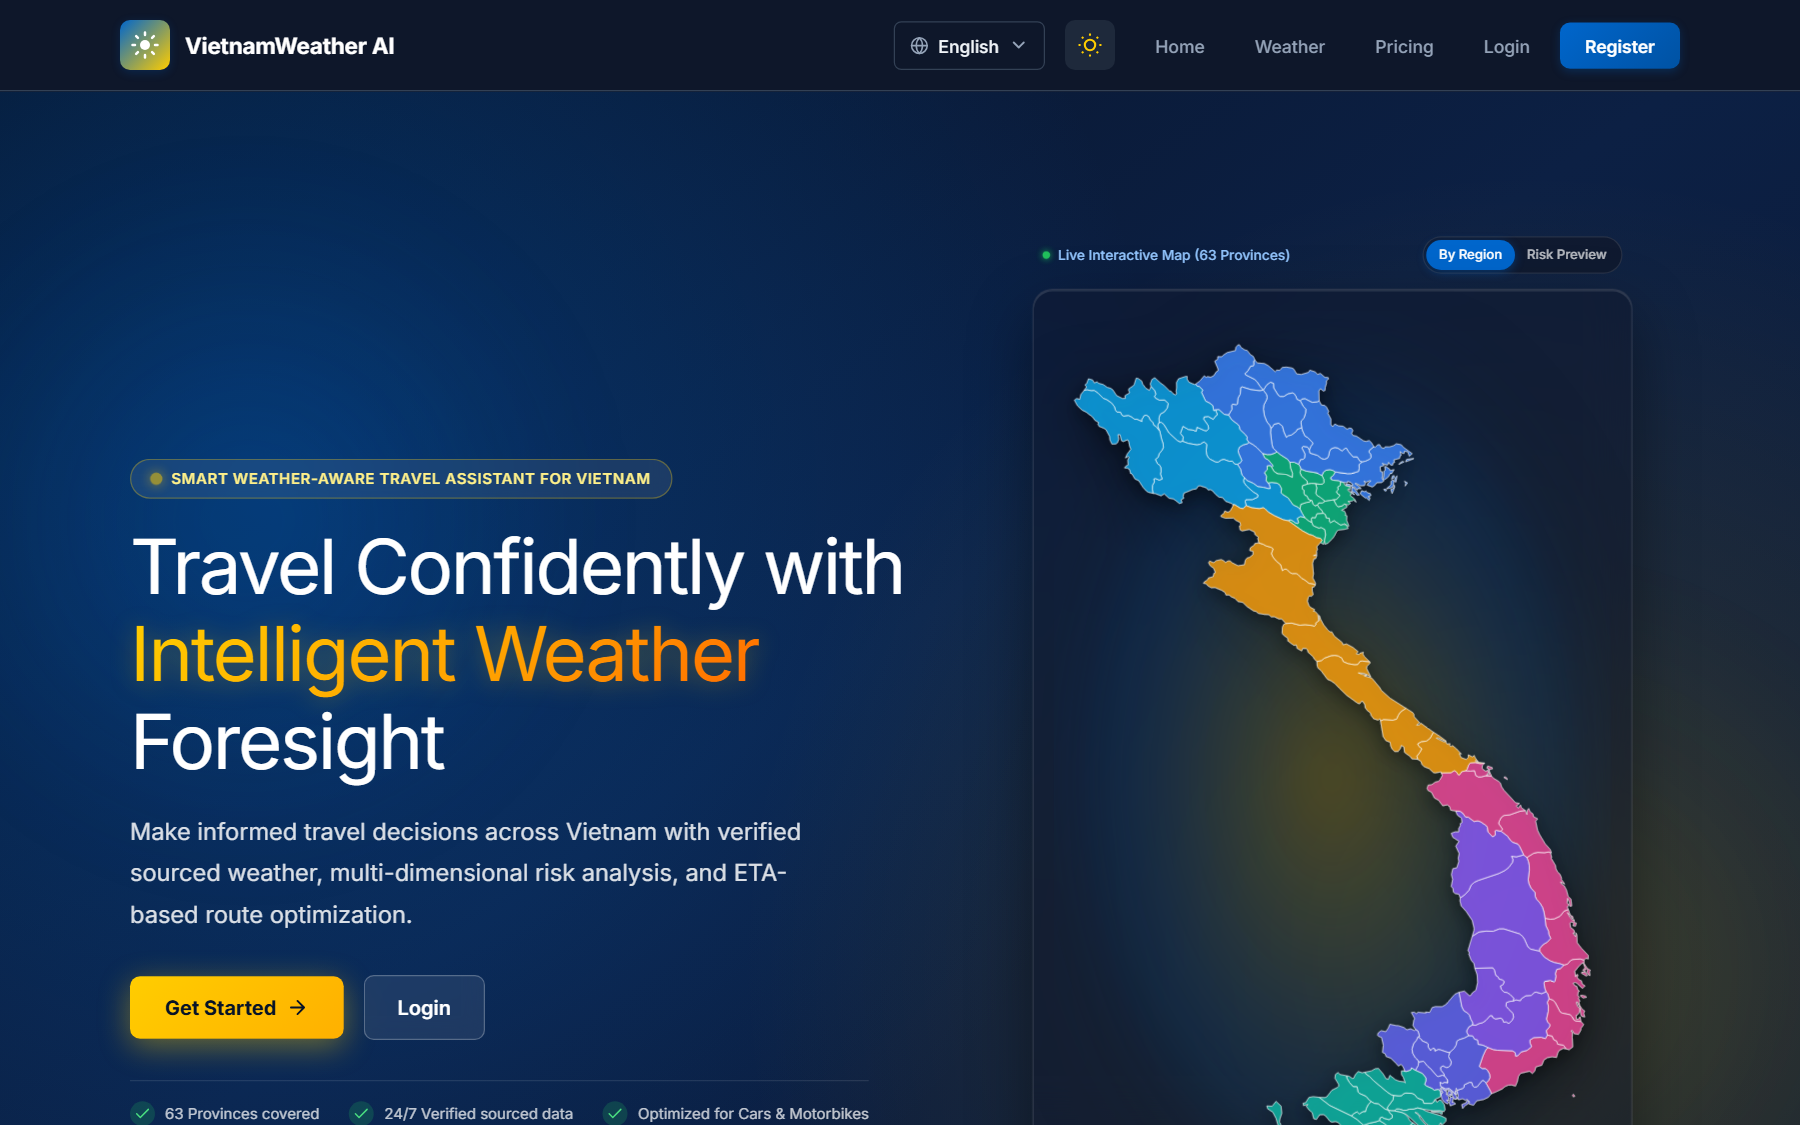
\includegraphics[width=0.88\textwidth, keepaspectratio]{figures/ui_landing.png}
\caption[VietForecast landing portal and nationwide meteorological gateway]{VietForecast landing portal and nationwide meteorological gateway in Dark Theme, introducing intelligent corridor planning and regional geography.}
\label{fig:ui_landing_en}
\end{figure}

\begin{figure}[htbp]
\centering
\begin{subfigure}[b]{0.48\textwidth}
    \centering
    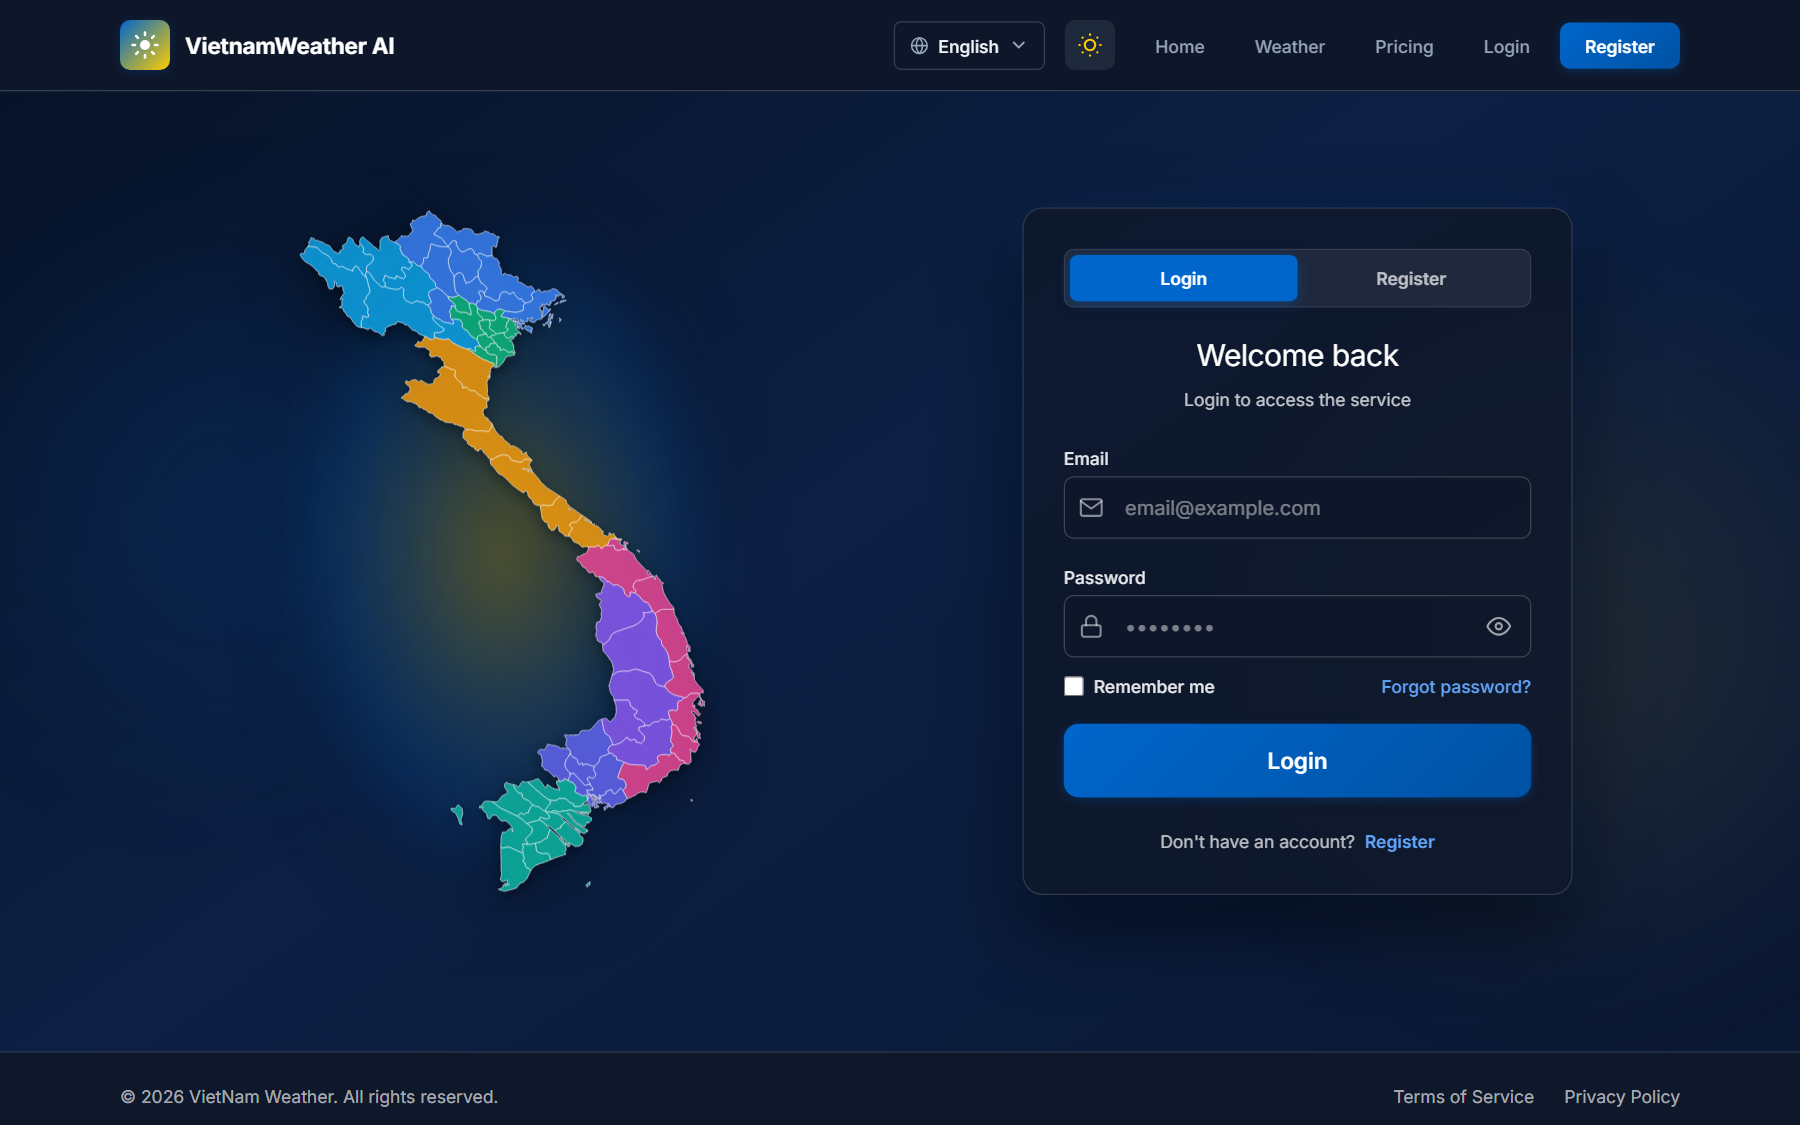
\includegraphics[width=\textwidth]{figures/ui_login.png}
    \caption{User Login Interface}
    \label{fig:ui_login_en}
\end{subfigure}
\hfill
\begin{subfigure}[b]{0.48\textwidth}
    \centering
    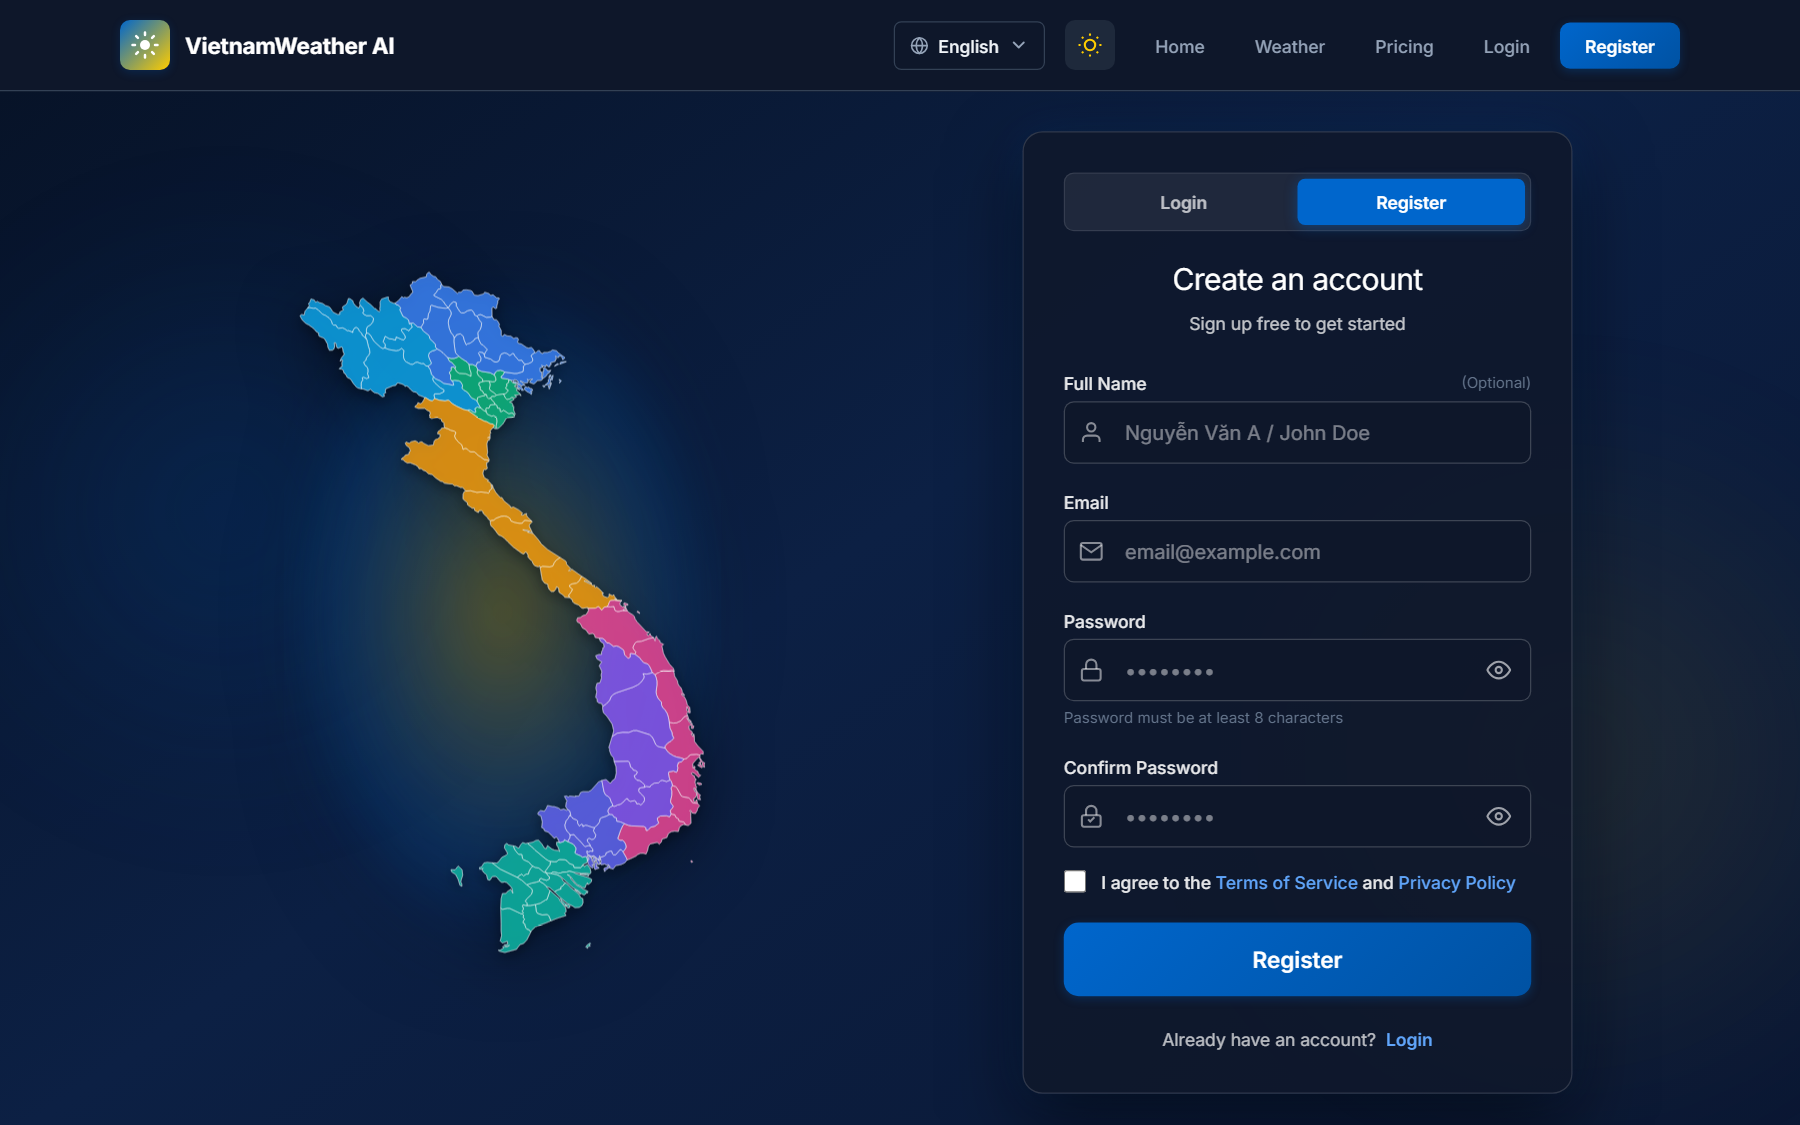
\includegraphics[width=\textwidth]{figures/ui_register.png}
    \caption{Account Registration Interface}
    \label{fig:ui_register_en}
\end{subfigure}
\caption[User Authentication and Identity Management Interface]{User Authentication and Identity Management interface subsystem (Login and Register) featuring a sleek Dark Theme, national geographic illustration, and robust session security compliant with ADR-004.}
\label{fig:ui_auth_en}
\end{figure}

\begin{figure}[htbp]
\centering
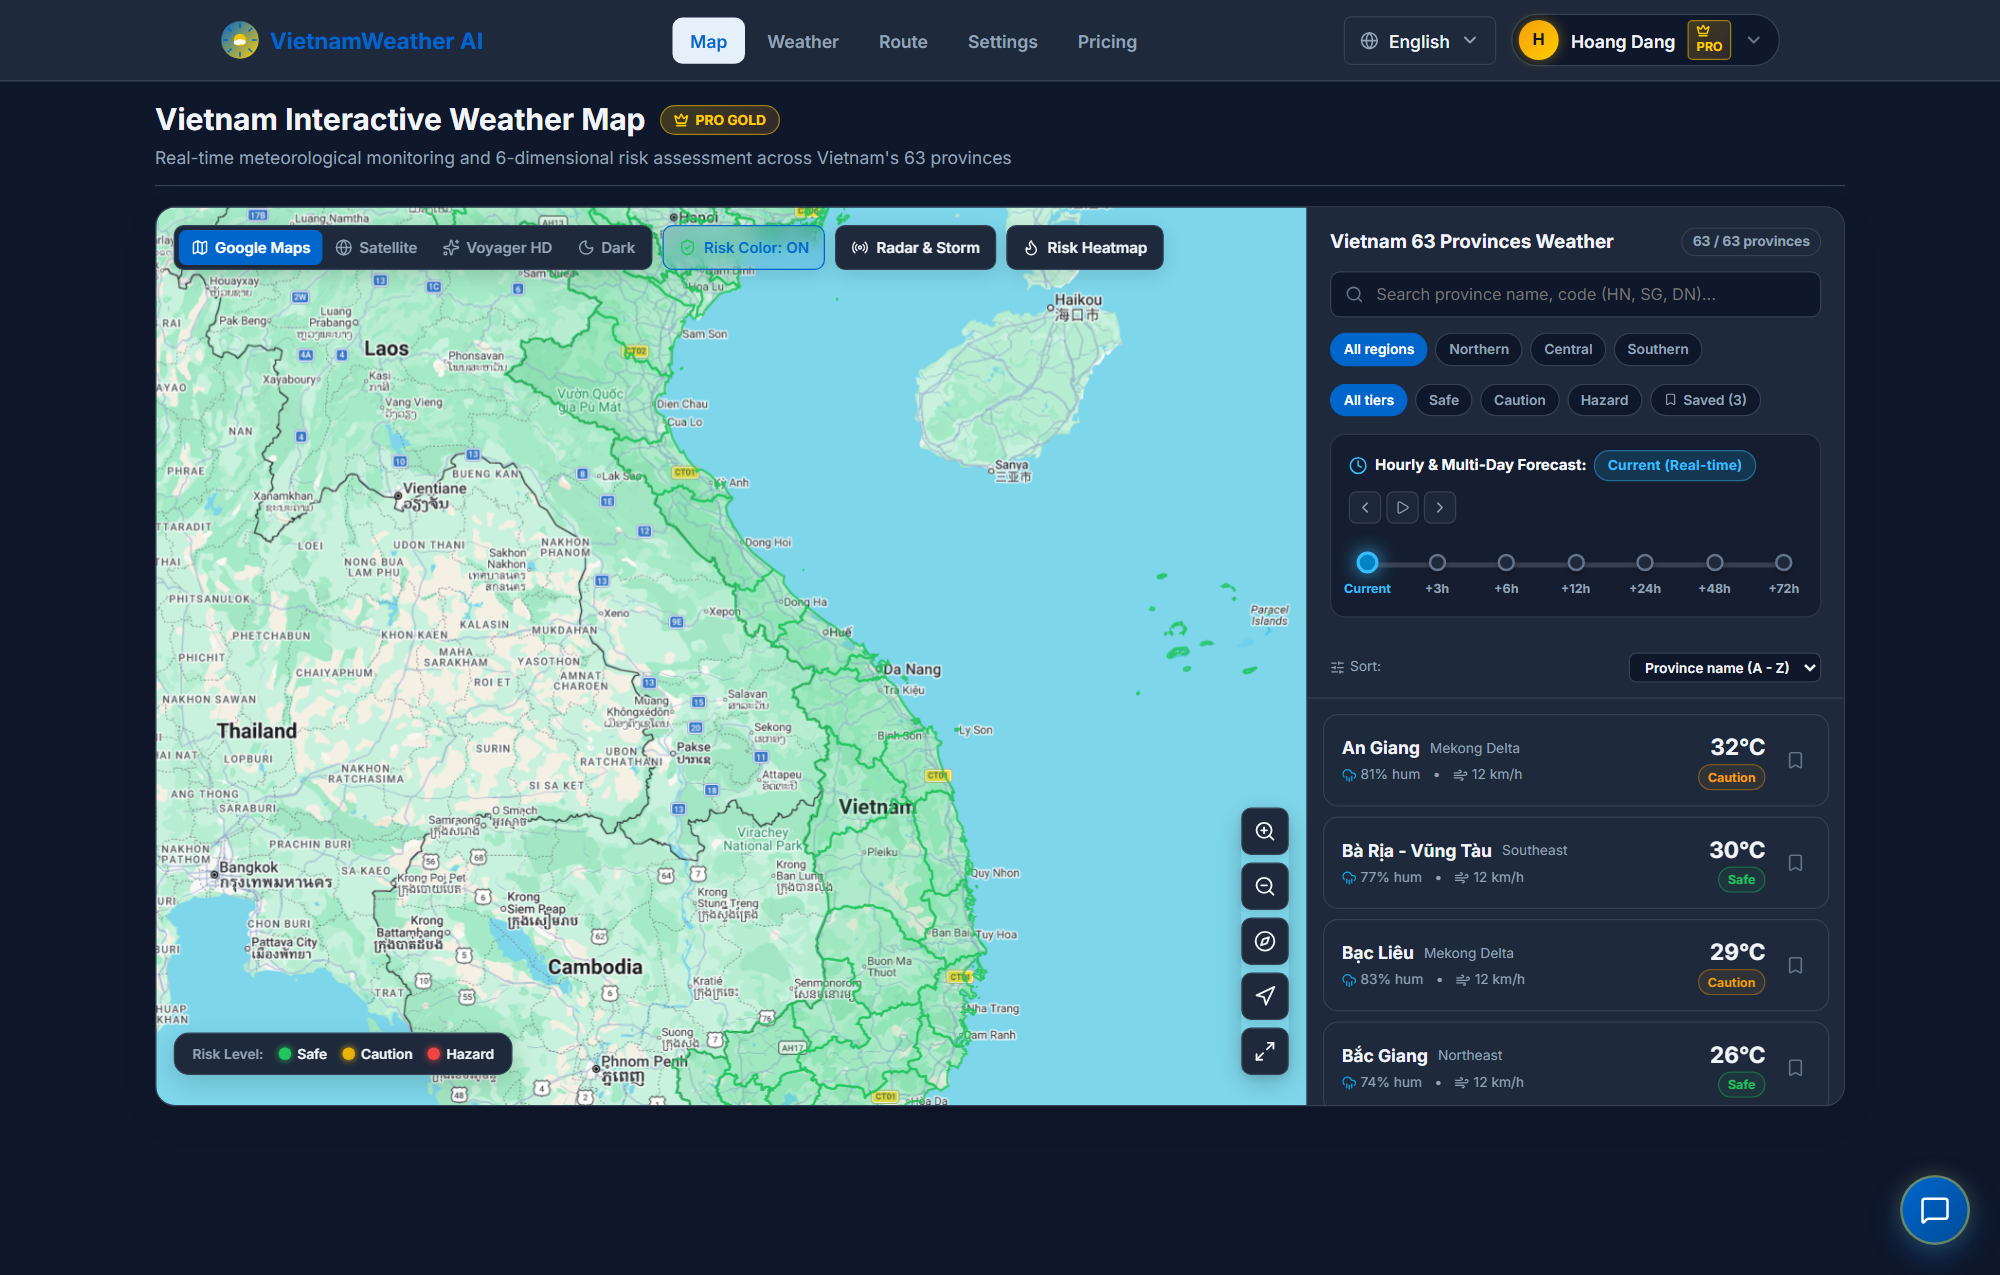
\includegraphics[width=0.88\textwidth, keepaspectratio]{figures/ui_map.png}
\caption[Interactive nationwide weather map across 63 provinces]{Interactive nationwide weather map across 63 provinces powered by Google Maps cartographic tiles, featuring an unobstructed canvas with hourly forecast filters cleanly integrated into the right-hand sidebar.}
\label{fig:ui_map_en}
\end{figure}

\begin{figure}[htbp]
\centering
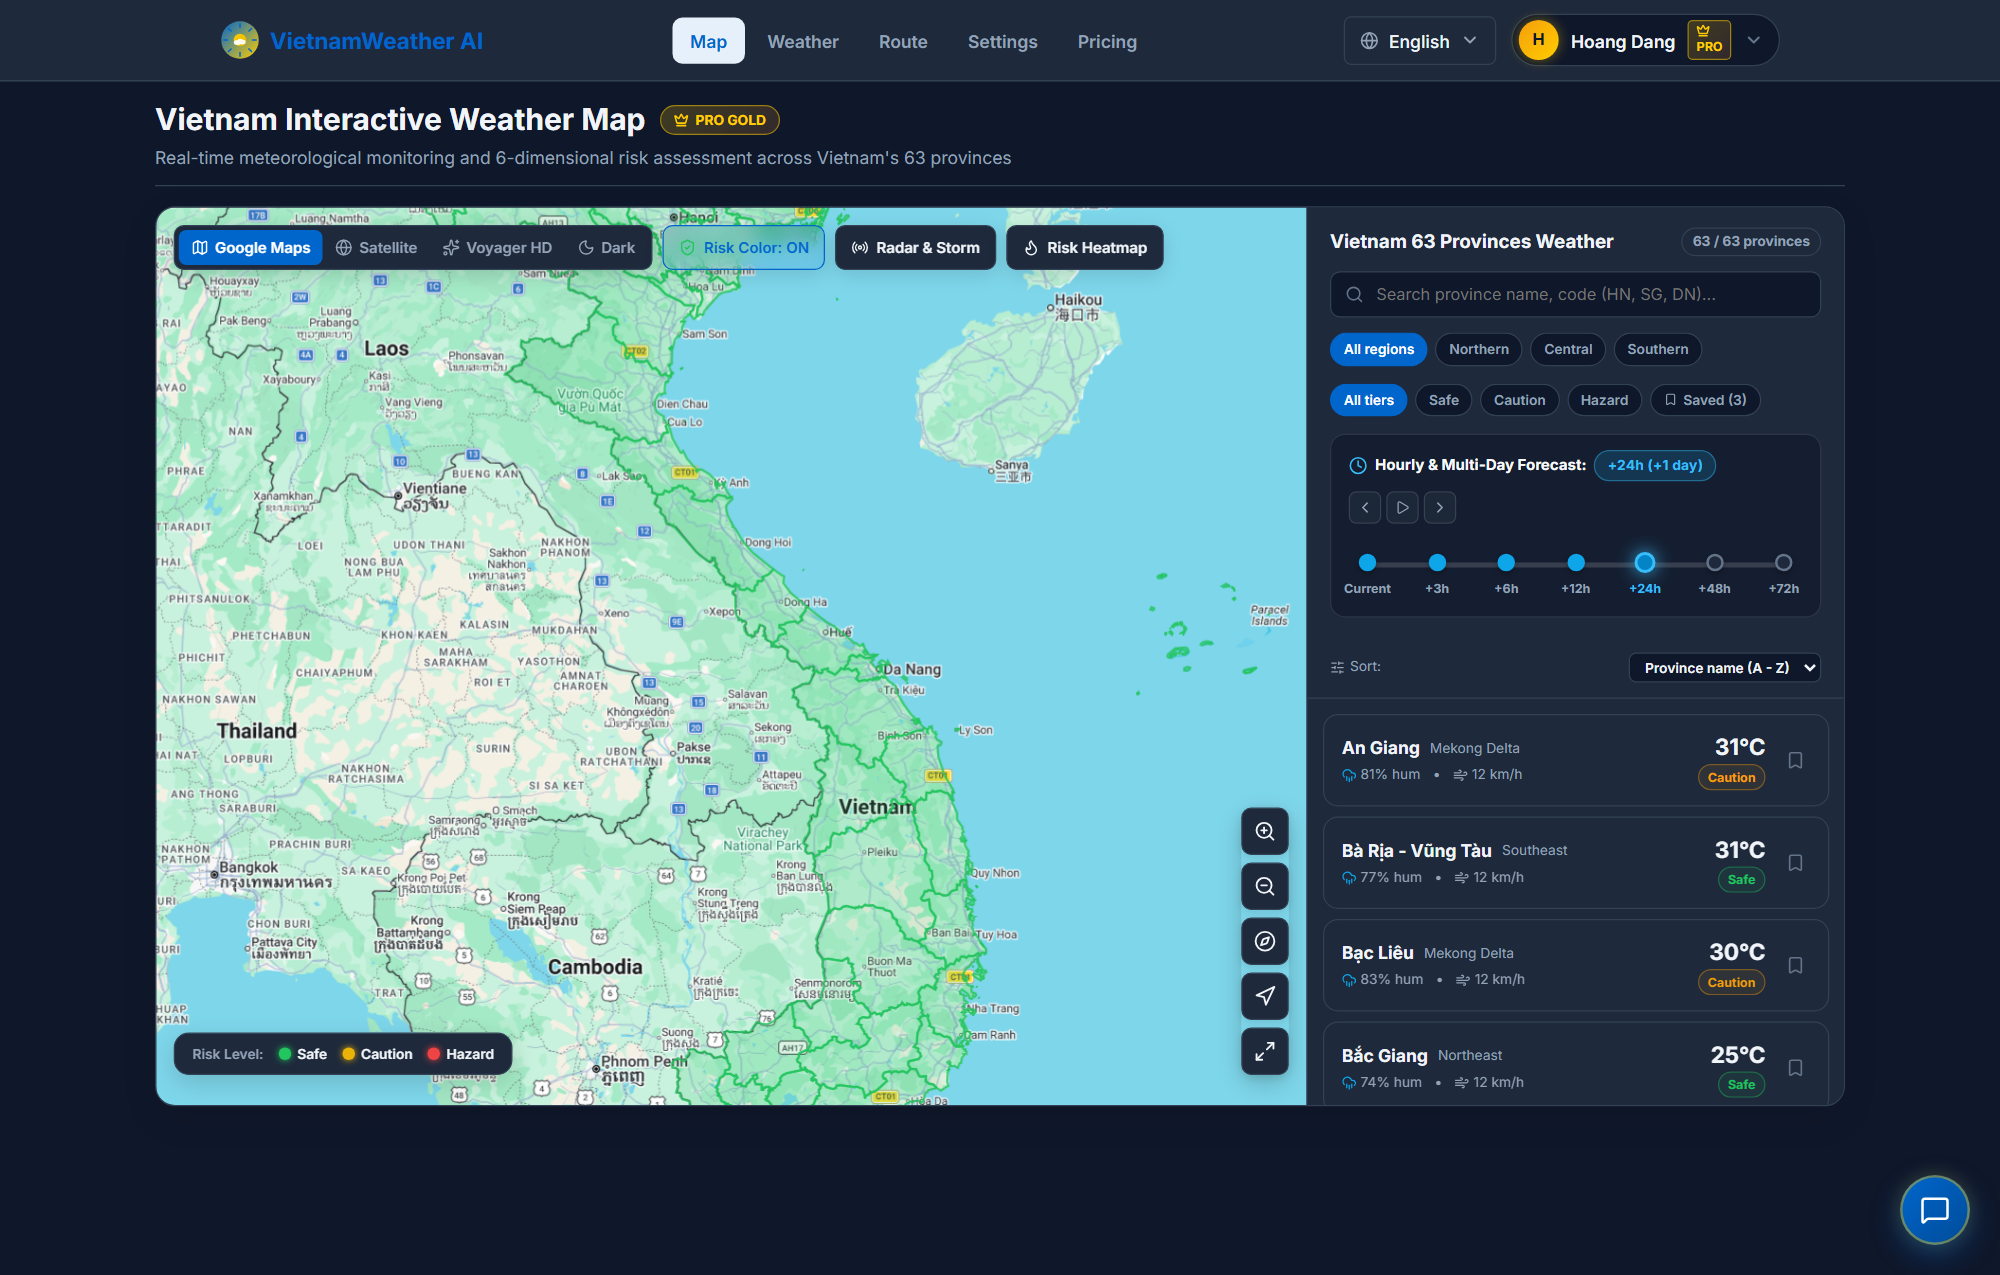
\includegraphics[width=0.88\textwidth, keepaspectratio]{figures/ui_map_timeline_slider.png}
\caption[Google Maps Weather Interface with Interactive Multi-Milestone Timeline Slider]{Google Maps meteorological interface with interactive linear timeline track slider in the sidebar, displaying simulation forecast at +24h (Next Day) on a PRO account.}
\label{fig:ui_map_timeline_slider_en}
\end{figure}

\begin{figure}[htbp]
\centering
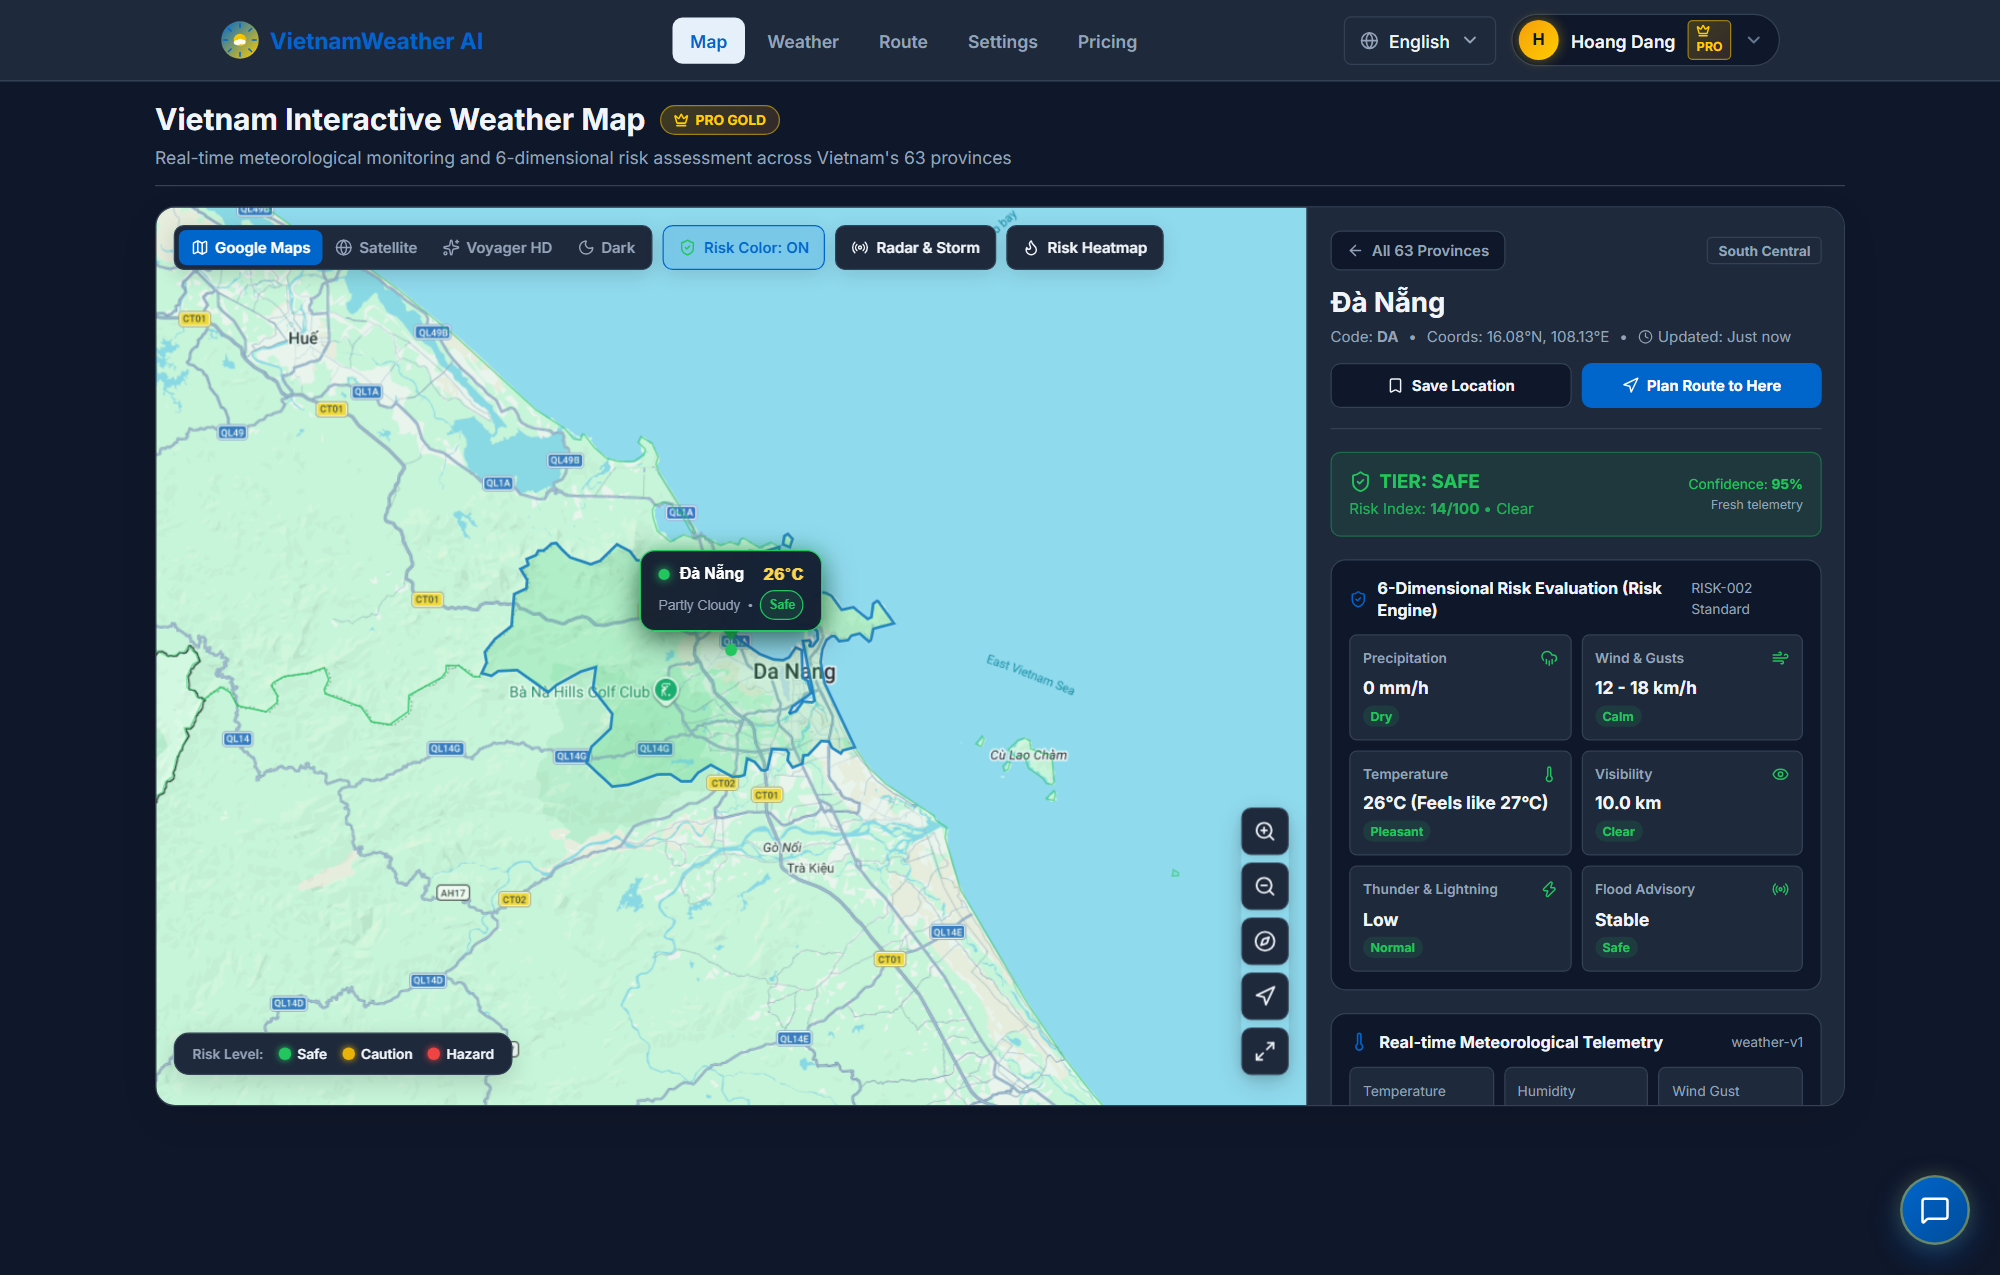
\includegraphics[width=0.88\textwidth, keepaspectratio]{figures/ui_map_detail.png}
\caption[Interactive provincial drill-down interface for Da Nang City]{Interactive provincial drill-down interface upon selecting Da Nang City: smooth WebGL camera zoom (\textit{flyTo}), administrative boundary neon highlight, anchored weather badge, and 6-dimension risk assessment matrix compliant with RISK-002.}
\label{fig:ui_map_detail_en}
\end{figure}

\begin{figure}[htbp]
\centering
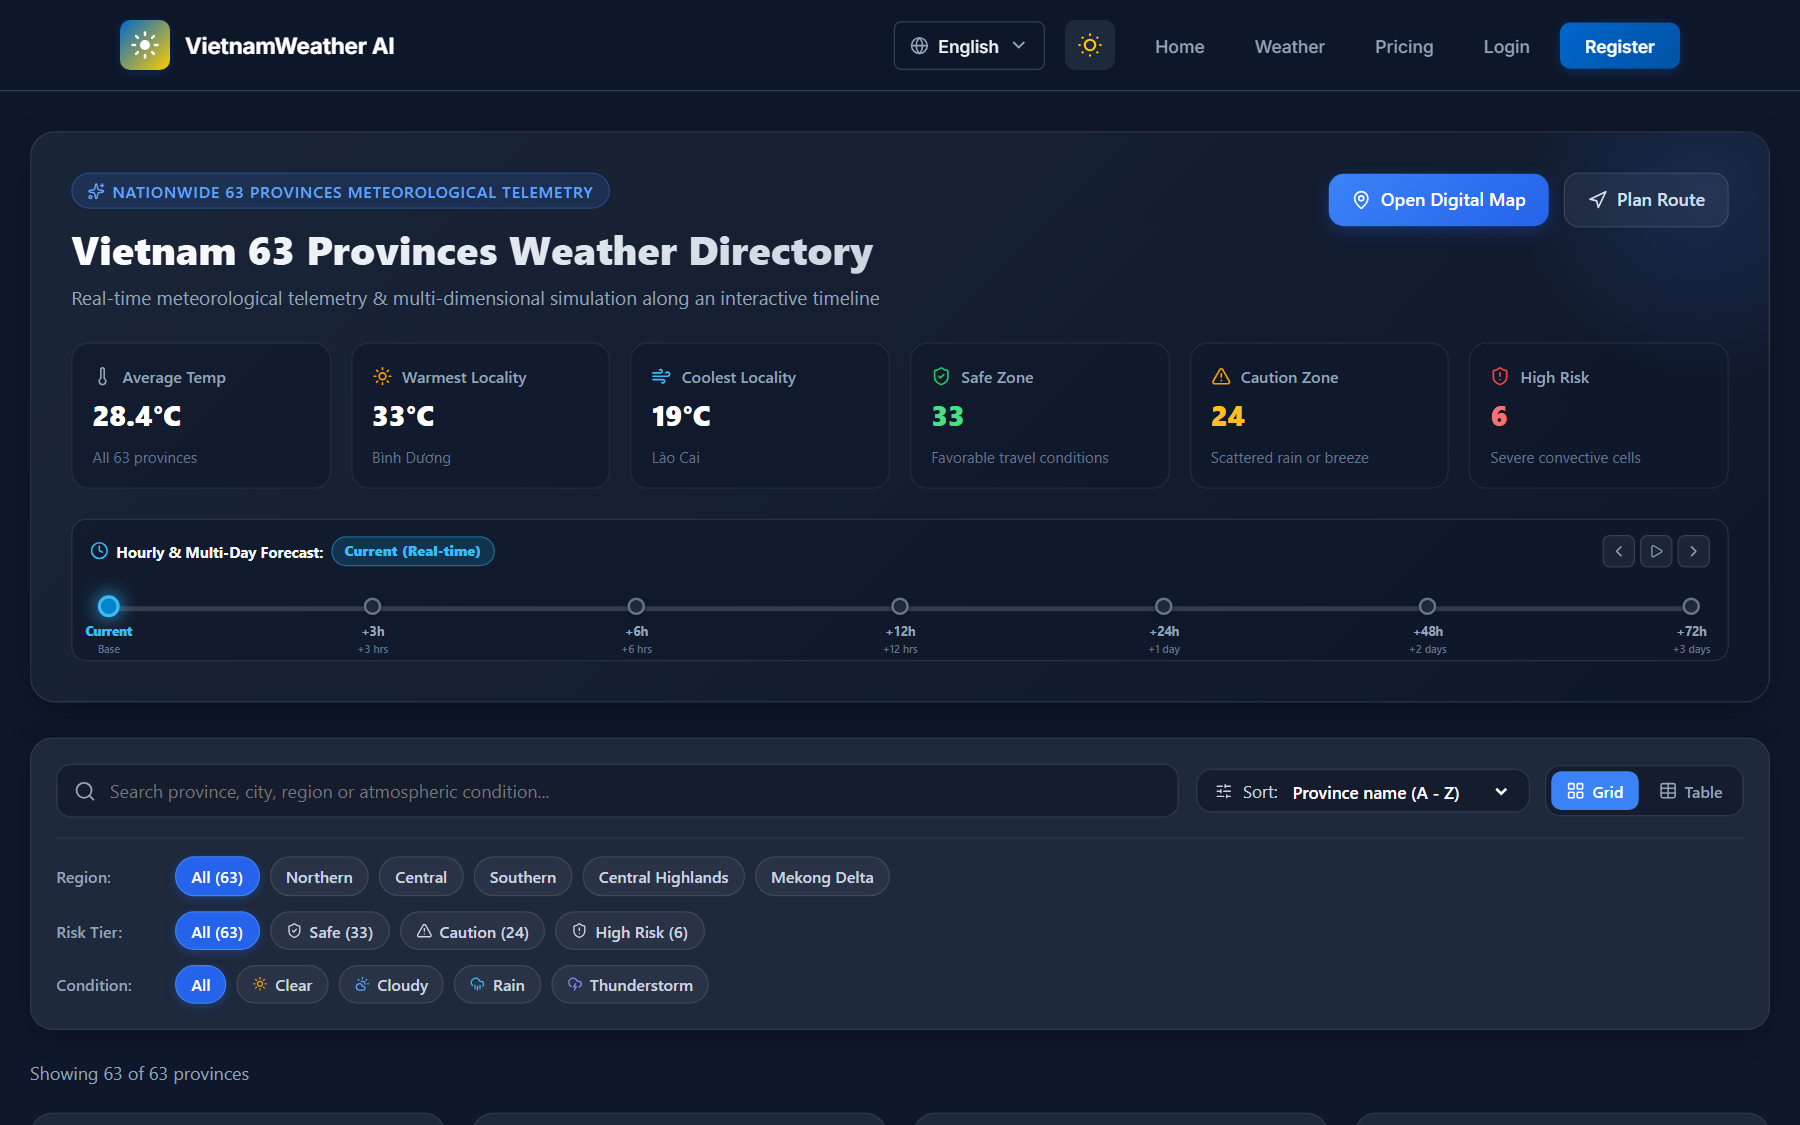
\includegraphics[width=0.90\textwidth, keepaspectratio]{figures/ui_weather_overview.png}
\caption[Dedicated Nationwide Weather Directory (63 Provinces)]{Dedicated Nationwide Weather Directory interface displaying national summary metrics, interactive draggable timeline slider (+24h as 1 day later), and multi-dimensional filter pills.}
\label{fig:ui_weather_overview_en}
\end{figure}

\begin{figure}[htbp]
\centering
\begin{subfigure}[b]{0.48\textwidth}
    \centering
    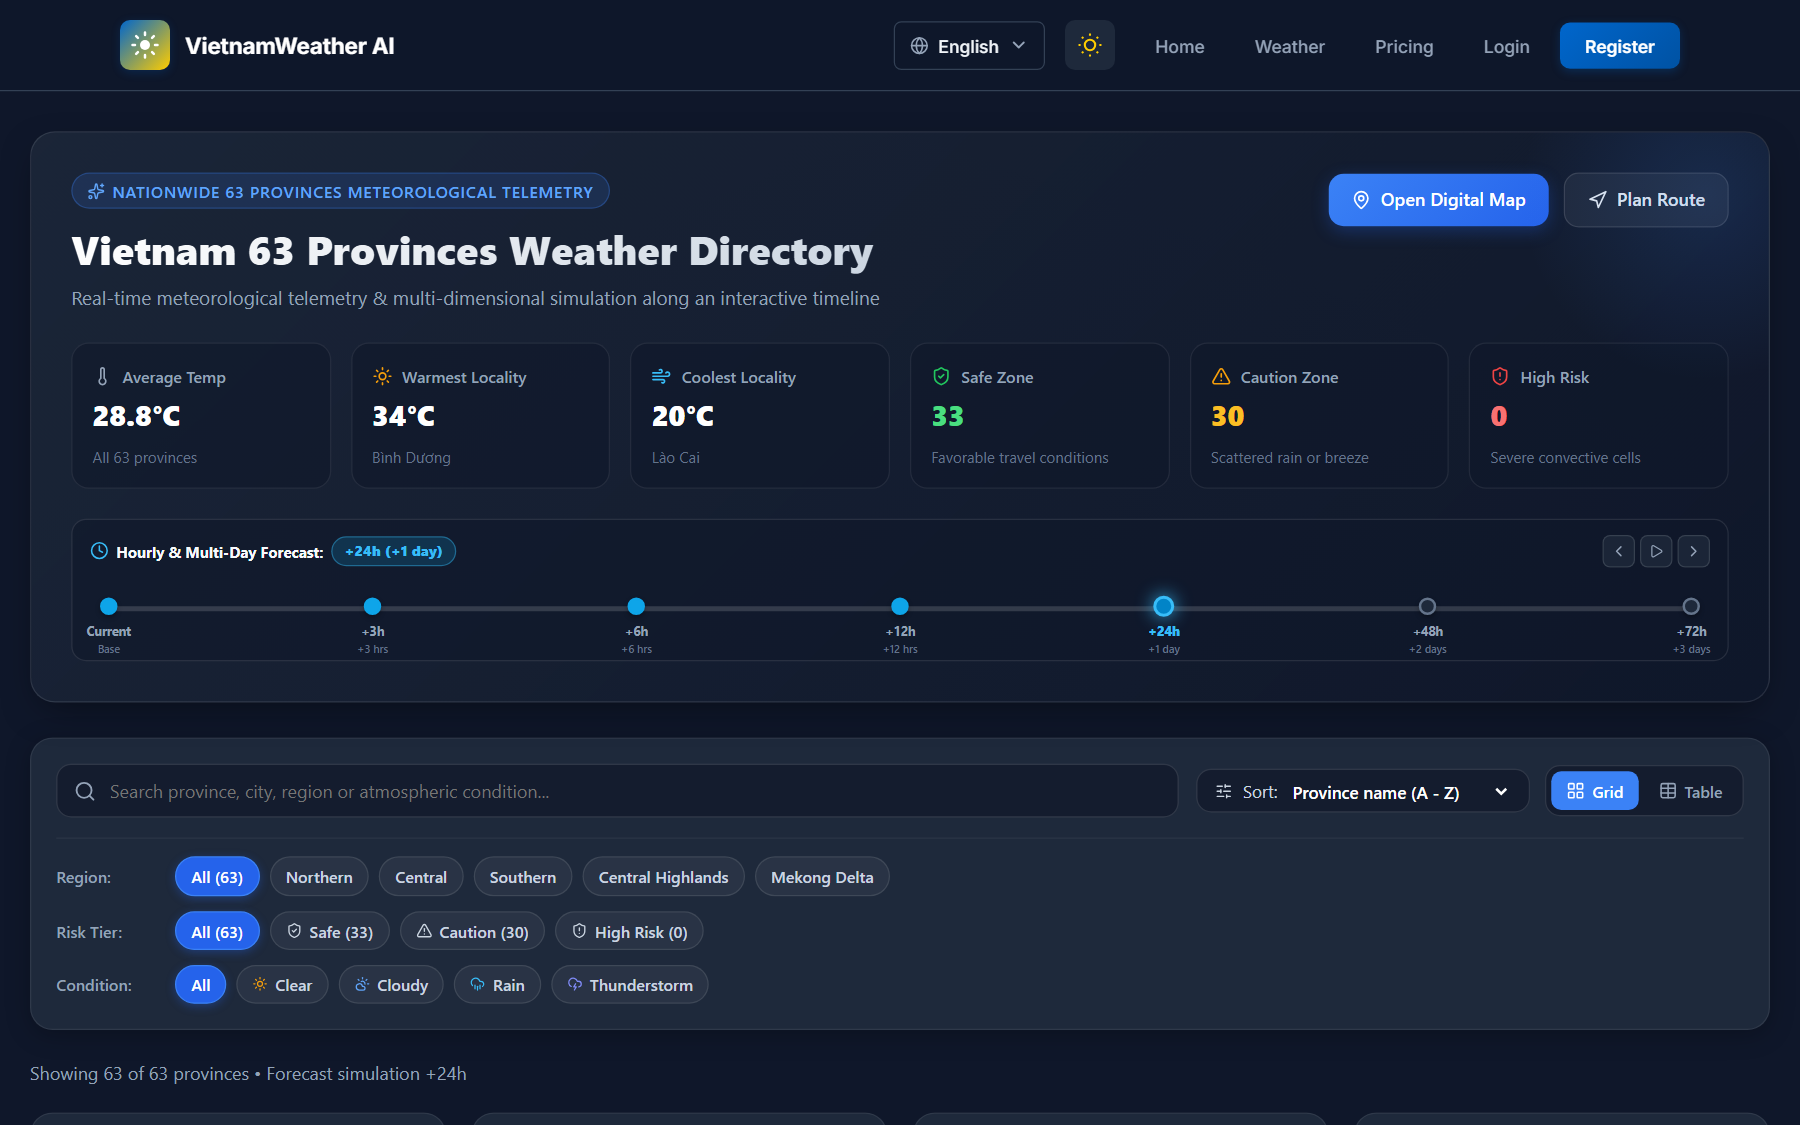
\includegraphics[width=\textwidth]{figures/ui_weather_timeline_24h.png}
    \caption{Scrubbing timeline to +24h (Next Day)}
    \label{fig:ui_weather_timeline_24h_en}
\end{subfigure}
\hfill
\begin{subfigure}[b]{0.48\textwidth}
    \centering
    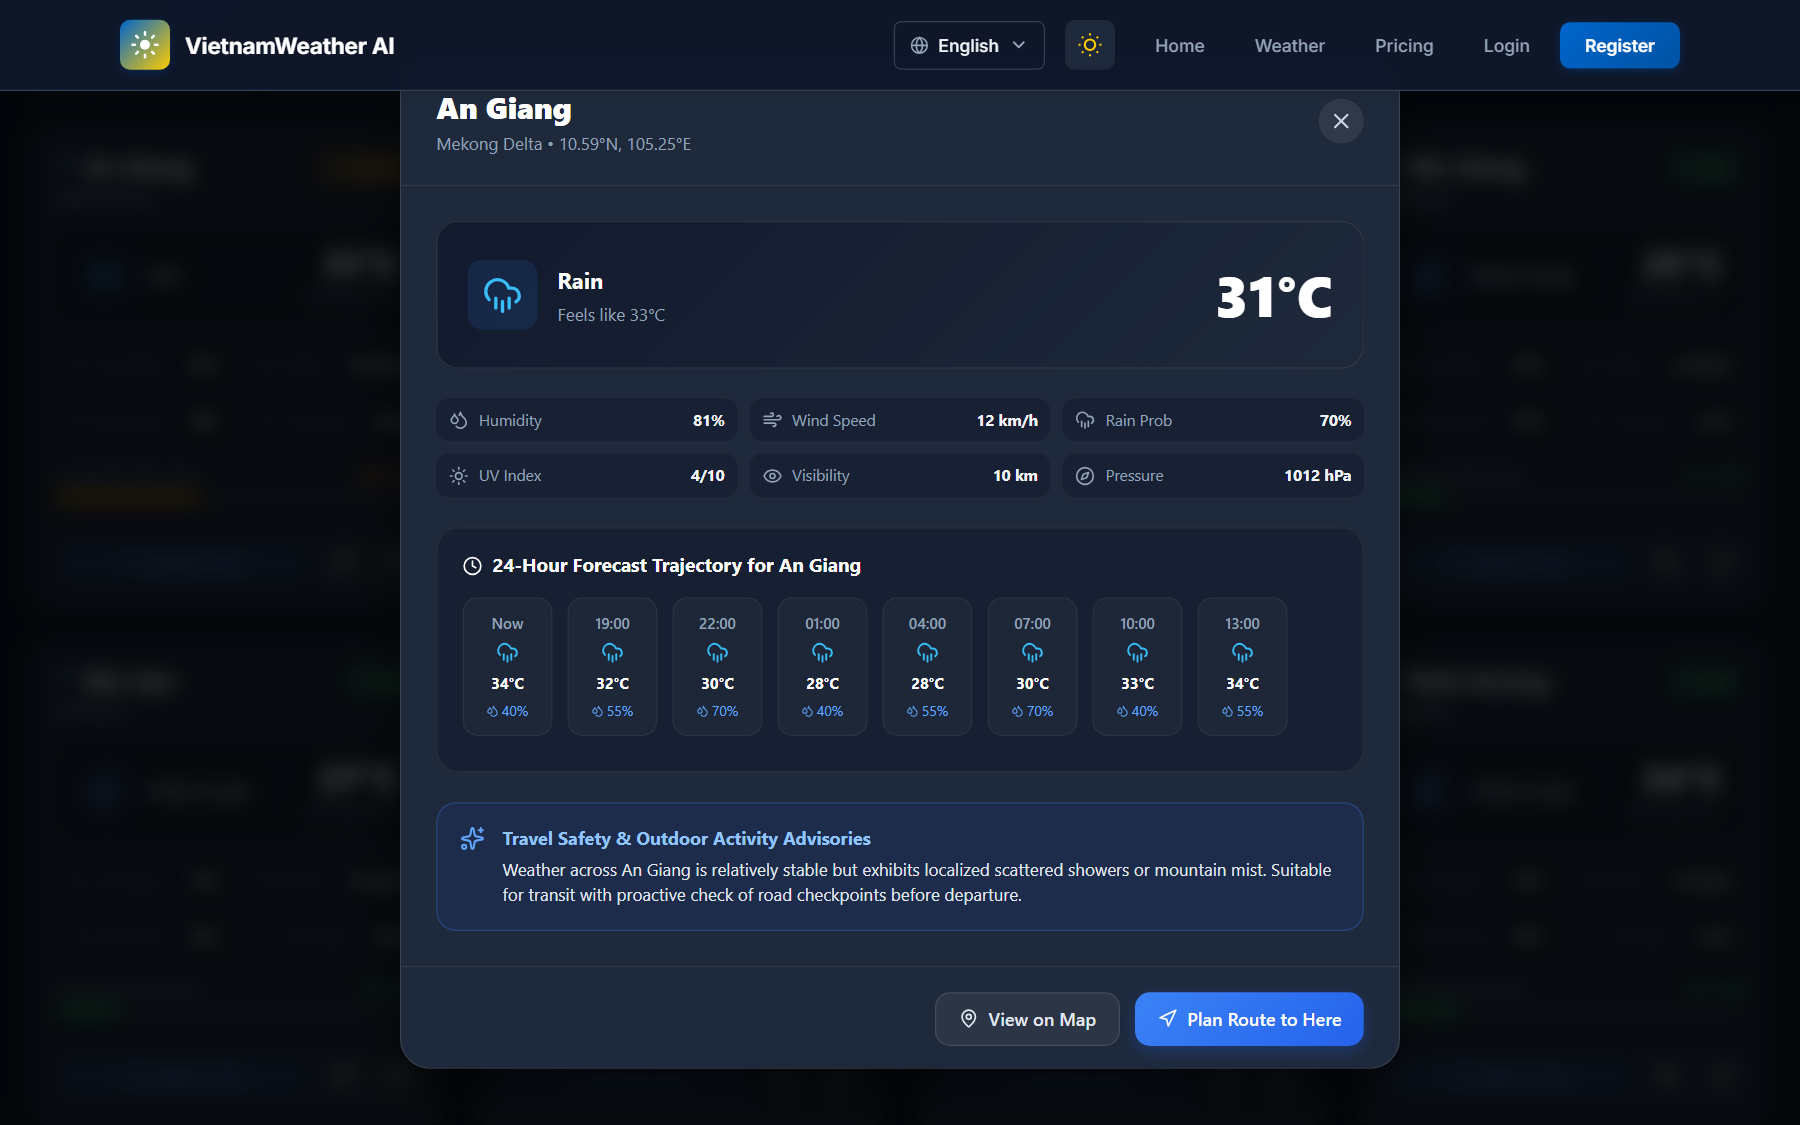
\includegraphics[width=\textwidth]{figures/ui_weather_modal.png}
    \caption{Provincial 24h trend and AI safety advisory}
    \label{fig:ui_weather_modal_en}
\end{subfigure}
\caption[Dedicated Weather Page Features and Provincial Drill-Down]{Dedicated Weather Page functionality: (a) Dynamic updates across 63 provinces upon scrubbing to +24h; (b) Provincial detailed micrometeorological dialog with 24-hour forecast trajectory and automated AI safety guidance.}
\label{fig:ui_weather_detail_features_en}
\end{figure}

\begin{figure}[htbp]
\centering
\begin{subfigure}[b]{0.48\textwidth}
    \centering
    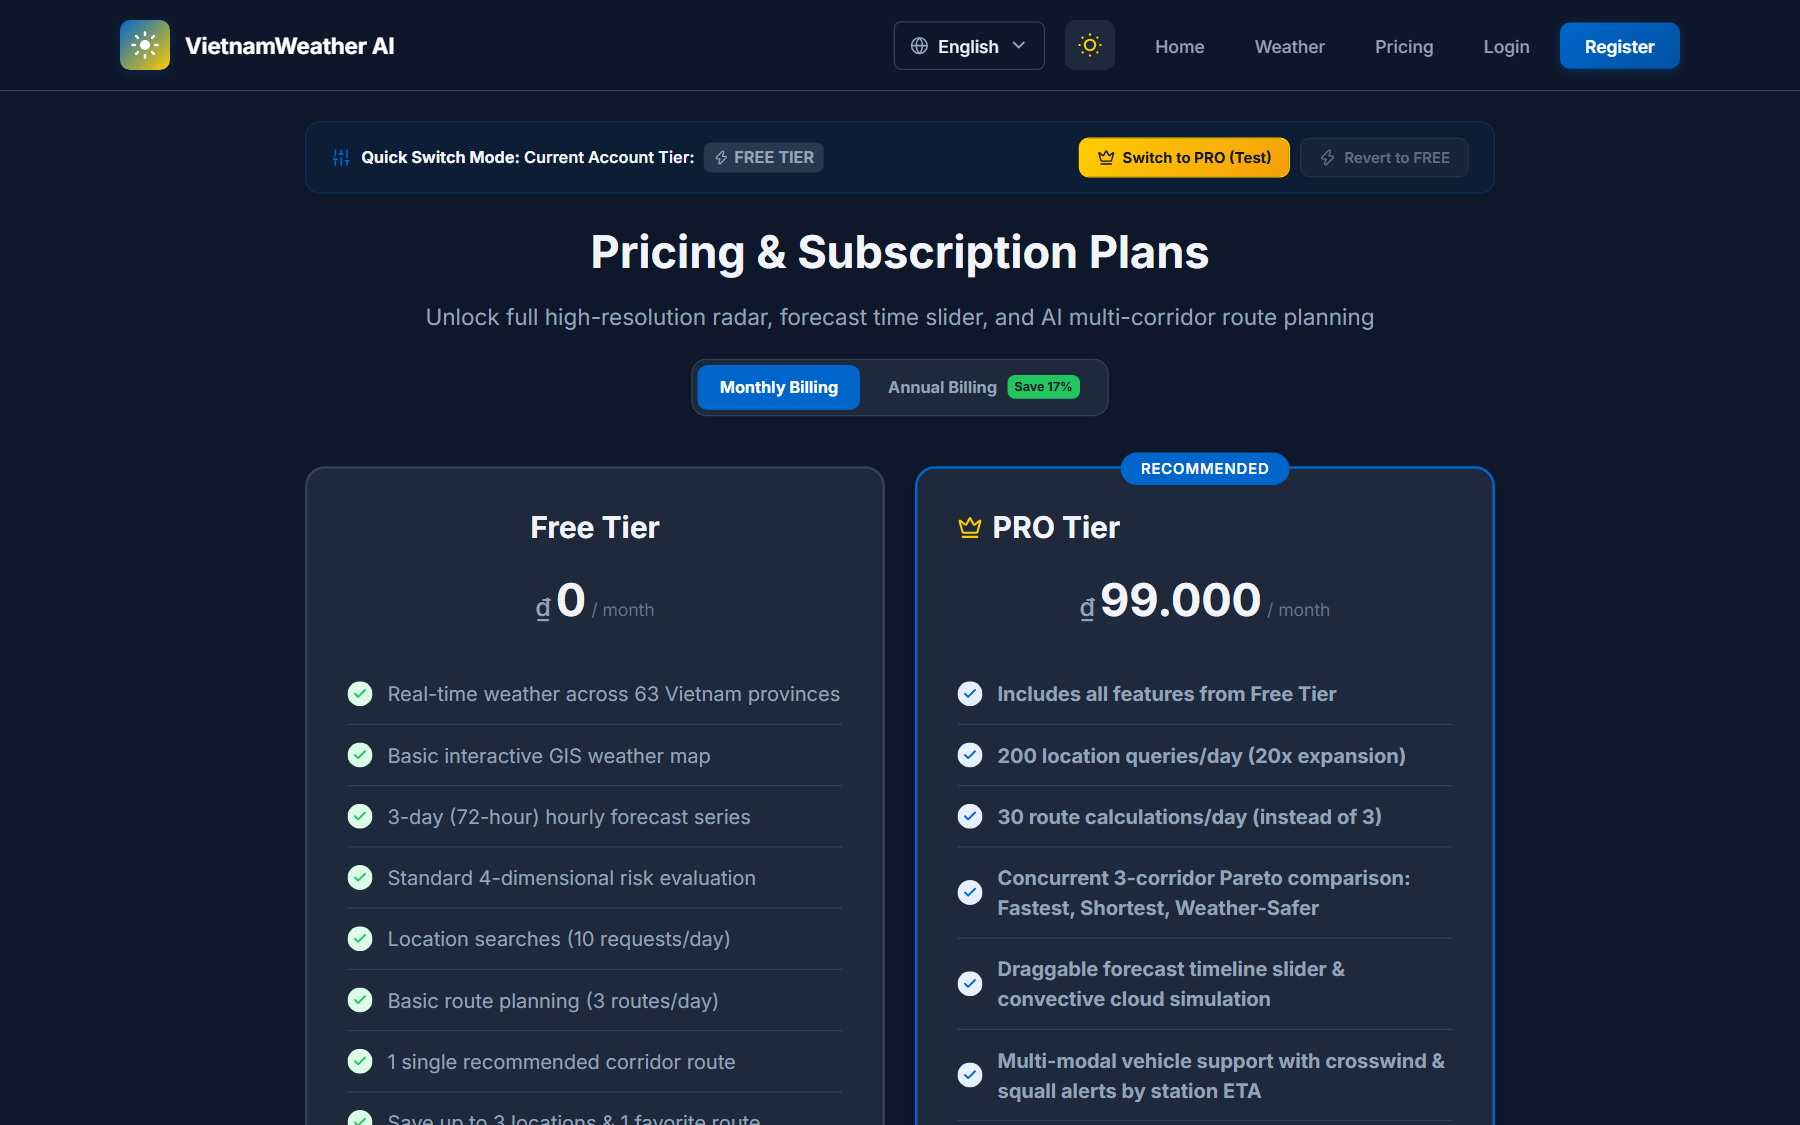
\includegraphics[width=\textwidth]{figures/ui_pricing.png}
    \caption{Plan Entitlements Comparison (Free vs. PRO)}
    \label{fig:ui_pricing_en}
\end{subfigure}
\hfill
\begin{subfigure}[b]{0.48\textwidth}
    \centering
    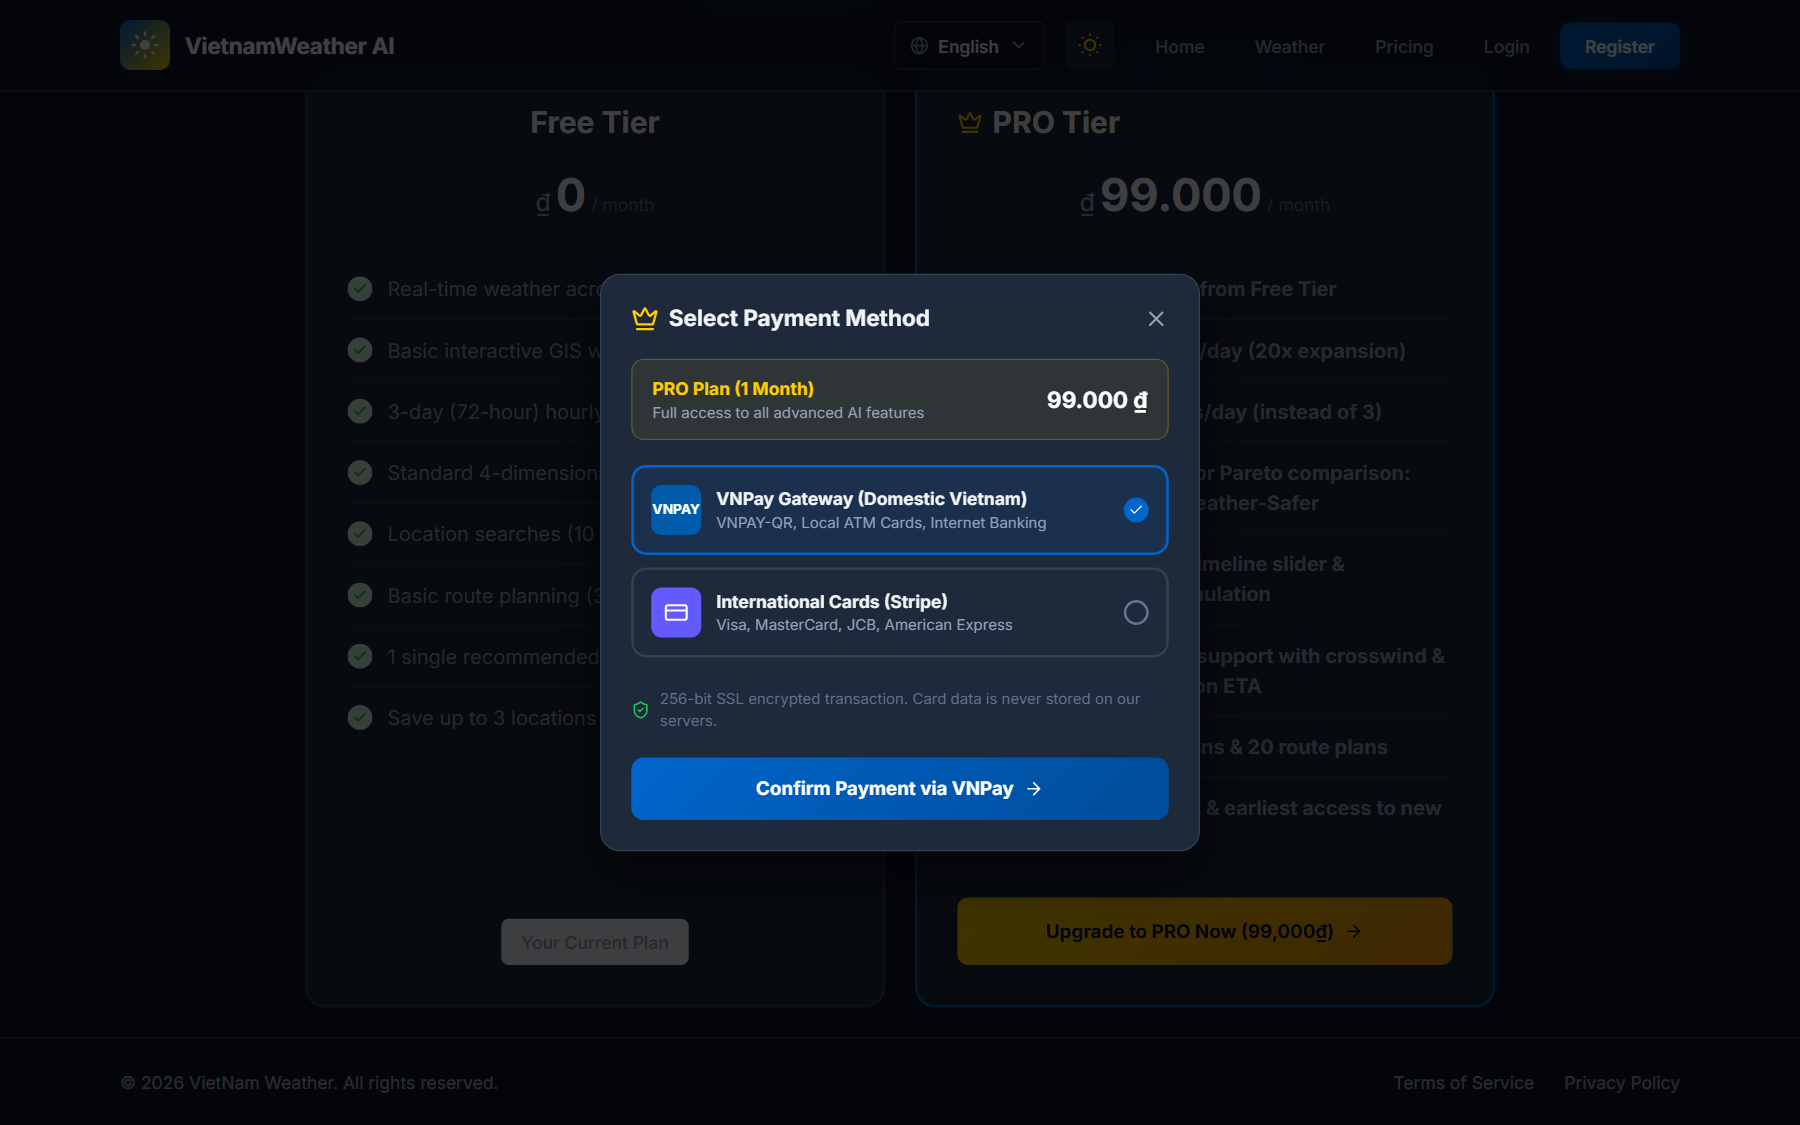
\includegraphics[width=\textwidth]{figures/ui_checkout.png}
    \caption{Multi-Gateway Checkout Modal (VNPay \& Stripe)}
    \label{fig:ui_checkout_en}
\end{subfigure}
\caption[Service pricing tiering and online payment checkout subsystem]{Service pricing tiering and online payment checkout subsystem of the VietForecast platform: (a) Comprehensive plan matrix comparing Free and PRO tiers with monthly/annual billing toggle; (b) Interactive checkout modal supporting domestic VNPay gateway (VNPAY-QR, ATM) and international Stripe gateway (Visa, MasterCard) protected by 256-bit SSL encryption.}
\label{fig:ui_monetization_en}
\end{figure}

\section{Chapter Summary}
\label{sec:evaluation_summary}

Chapter~\ref{ch:evaluation} has documented the experimental evaluation of the VietForecast platform, demonstrating significant empirical achievements:
\begin{itemize}
    \item[-] \textit{Routing safety}: The Weather-Safer algorithm eliminated $87.2\%$ of severe weather hazard checkpoints across three representative corridors, while strictly bounding travel duration overhead to $8.9\%$ and distance expansion to $4.7\%$. Vehicle-differentiated calibration successfully alerted motorcyclists to hazardous crosswinds.
    \item[-] \textit{System performance}: Two-tier PostGIS GiST indexing reduced corridor query latency to $11.4$~ms on 100,000 stations ($36.9\times$ faster than sequential scanning). The Fastify API achieved $> 2,485$~req/s with $p_{95} = 12.8$~ms and zero 5xx errors. The circuit breaker safely isolated third-party faults within 60 seconds.
    \item[-] \textit{Artificial intelligence}: The AI assistant attained $96.2\%$ tool dispatch accuracy, $97.2\%$ empirical citation grounding, suppressed factual hallucination to $1.8\%$ (a $94.8\%$ reduction versus ungrounded baselines), and delivered a $2.2$~ms deterministic fallback response during external outages.
    \item[-] \textit{User experience}: The WebGL interface scored an outstanding $84.6/100$ on the System Usability Scale (Grade A / Excellent), confirming strong operational acceptance.
\end{itemize}

These empirical findings validate the initial research and engineering hypotheses, establishing a firm scientific foundation for the conclusions and future directions presented in Chapter~\ref{ch:conclusion}.
